\documentclass[a4paper, 10pt, openany]{book} %chose the paper size and font size. Openany ensures that all all chapters and similar may begin at any page, not only odd pages. For the introductory pages and appendices we want openany, but for chapter pages in the main content we want chapters to begin only on odd pages (right hand side). The book class ensures that the margins are automatically adjusted such that left hand pages are slightly moved to the left and vice versa at the right, which makes the thesis very readable and good looking when printed in bound book format.
%\usepackage[utf8]{inputenc} %to manage special characters
\usepackage[T1]{fontenc} %to manage special characters
\usepackage[Bjarne]{fncychap} %fancy chapter style (many more available, like Sonny or Lenny etc.)
\usepackage{fancyhdr} %to customize the headers
\usepackage[lmargin=1.5in, rmargin=1in, tmargin=1in, bmargin=1in] {geometry} %sets the margins for the pages
\setcounter{tocdepth}{2} %table of contents number depth for subsections (2 = x.x.x)
\setcounter{secnumdepth}{4} %numbering depth for headers for subsections in the text(4 = x.x.x.x)
\usepackage{url} %to include urls
\usepackage{listings} %include this if you want to include code in the thesis
\usepackage{amsmath,amssymb} %mathematical package
\usepackage{siunitx} %includes SI-units
%\usepackage{caption}
%\captionsetup{font=bf}
%\makeatletter
%\renewcommand*\l@figure{\@dottedtocline{1}{1.5em}{3em}}
%\renewcommand*\l@table{\@dottedtocline{1}{1.5em}{3em}}
%\makeatother
\usepackage[bf]{caption} %makes float captions bold
\usepackage{array}
\usepackage{booktabs}
\usepackage{graphicx} %to include graphics
\usepackage{float} %to include floats
\usepackage[export]{adjustbox} %to adjust floats
\usepackage{subfig} %to include subfigures
\usepackage{tikz} %for inline diagrams
\usetikzlibrary{arrows.meta, positioning}
\usepackage{chngcntr} %will make it possible to change the counter for tables, figures etc. such as below
\counterwithin{figure}{section} %change counter for figures within sections (also possible to choose for each chapter
\counterwithin{table}{section} %change counter for tables within sections
\usepackage{color, xcolor} %edit e.g. text colors
\usepackage{setspace}
\setstretch{1.15}
\raggedbottom % prevent book-class flushbottom from stretching gaps between short sections
\usepackage{parskip}
\usepackage{iftex}
\ifXeTeX
  \usepackage{fontspec}
  \setmainfont{Verdana}
\fi
\frenchspacing % uniform spacing after sentence-ending periods (removes the wide "double space" look after periods)

% Tighten the vertical spacing around section headings (default book-class gaps look large with parskip).
% If headings ever look wrong, simply remove this titlesec block.
\usepackage{titlesec}
\titlespacing*{\section}{0pt}{2ex plus 1ex minus .2ex}{1ex plus .2ex}
\titlespacing*{\subsection}{0pt}{1.5ex plus .5ex minus .2ex}{0.6ex plus .2ex}
\titlespacing*{\subsubsection}{0pt}{1.2ex plus .5ex minus .2ex}{0.5ex plus .2ex}


\usepackage[backend = biber,
            style = numeric,
            date = long,     % Long: 24th Mar. 1997 | Short: 24/03/1997
            sorting = none,
            maxcitenames = 3,   % max names to include before et. al.
            ]{biblatex} %customize the look of your citations and bibliography
\addbibresource{bibliography.bib} %declare the bibliography resource
\usepackage{comment} %to be able to comment out sections in the .tex files
\usepackage{pdfpages} %to include external PDF files in appendices
\usepackage{afterpage} %to customize page commands such as below
\newcommand\myemptypage{
    \null
    \thispagestyle{empty}
    \addtocounter{page}{-1}
    \newpage
    } %sets new page command to insert an empty page without adding to the page counter or having a page number
\usepackage[colorlinks=true,linkcolor=black, citecolor=black]{hyperref} % For clickable links
\usepackage[acronym, toc]{glossaries} % For glossary and abbreviations

\makenoidxglossaries % noidx mode: builds the Abbreviations/Terms lists from the normal xelatex passes
                     % (matches \printnoidxglossary in 02Abbreviations.tex / Terms.tex; no makeglossaries step needed)

\loadglsentries{glossary}




% --- Fix List of Figures / List of Tables number width. Figures and tables are section-numbered
% (e.g. 2.15.1), which overflows the default number box and makes the number overlap the caption text.
% Widen the number box. Placed at the end of the preamble so subfig/hyperref do not override it. ---
\makeatletter
\renewcommand*\l@figure{\@dottedtocline{1}{1.5em}{3.8em}}
\renewcommand*\l@table{\@dottedtocline{1}{1.5em}{3.8em}}
\makeatother

\begin{document}
%%%%%%%%%%%%%%%%%%%%%%%%%%%%%%%%%%%%%%%%%%%%%%%%%%%%%%%%
%\begin{comment}
% The title page:
% For NTNU students this page will be generated automatically when submitting your paper, and should not be included in the final file from Latex. Delete or comment out the title page setup. The final report should then start with the first page being the abstract. I have included a title page here so it is possible to see how it may look like, and for those who does not get an automatically generated title page. Of course you will need to change the names and titles etc. to your case.

%the title page should be an odd page (right hand side)

\begin{titlepage}
\newgeometry{left=1.6in, right=2in}
\vspace*{1.5cm}

\noindent  \textcolor{gray}{\large Aleksander Nesvik, Daniel Alnes} \\
\vspace{1cm}

\noindent \textbf{\Large Visualization of Automatic Identification System Messages for the Norwegian Coastal Administration} \\
\vspace{0.5cm}

\noindent {\large Towards a safer and more secure ocean for Norway} \\



\vspace{7cm}
\noindent Bachelor's thesis in Computer Engineering \\
Supervisor: Di Wu \\
May 2026 \\

\vspace{0.2cm}
\noindent Norwegian University of Science and Technology \\
Faculty of Information Technology and Electrical Engineering \\
Department of ICT and Natural Sciences \\

\begin{figure}[h]
    
\includegraphics[width=0.28\textwidth]{Figures/ntnu_basic.png}
\end{figure}
\end{titlepage}
\restoregeometry
\myemptypage %empty page such that the abstract starts at the first right hand side after the title page
%\end{comment}
%%%%%%%%%%%%%%%%%%%%%%%%%%%%%%%%%%%%%%%%%%%%%%%%%%%%%%%%

% The pre-chapters
\chapter*{Abstrakt}
\pagenumbering{roman} %introductory pages should be roman
\setcounter{page}{1}
\addcontentsline{toc}{chapter}{\protect\numberline{}Abstrakt} %add the chapter to the table of contents, this is not automatically added when creating unnumbered chapters (*). Add it in a chapter style, and keep all chapters on the same numberline indent regardless of number or not on the chapter

Dette prosjektet ble gjennomført i samarbeid med Kystverket. Målet med prosjektet var å utforske og evaluere alternative visualiseringsteknikker for store datasett, samt å teste om slike visualiseringsmetoder kunne gi verdi for kunden.

Systemet ble utviklet som en applikasjon med en hjemmeside. React og TypeScript ble brukt for å lage applikasjonen, med MapLibre GL JS som basiskart og Deck.gl som datavisualiseringslag. Backend ble levert av kunden, og REST API-endepunkter ble brukt for å hente data som frontend visualiserer.

Flere visualiseringsmetoder ble implementert, inkludert klynging, varmekart, signalstyrkevisualisering og visualisering av anomaligrupper. Disse ble brukt til å evaluere hvor effektivt slike metoder kan forenkle store datasett til visuelt forståelige representasjoner.

Resultatene viser at kombinasjonen av flere ulike visualiseringsmetoder kan gi bedre innsikt for maritime operatører. Gruppen fikk positive tilbakemeldinger på den implementerte løsningen. Dette viser at prototyping med open source-verktøy og testdata kan gi verdi før full produksjon av slik funksjonalitet blir laget for interne verktøy, slik at man kan evaluere om funksjonaliteten gir verdi før produksjon. 



\chapter*{Abstract} %pre-chapters should not be numbered, hence the "*"
\addcontentsline{toc}{chapter}{\protect\numberline{}Abstract} %add the chapter to the table of contents, this is not automatically added when creating unnumbered chapters (*). Add it in a chapter style, and keep all chapters on the same numberline indent regardless of number or not on the chapter

This project was conducted in collaboration with the Norwegian Coastal Administration. The aim of the project was to explore and evaluate alternative visualization techniques for large-scale datasets, to assess whether such visualization methods would provide value to the customer. 

The system was developed as a single-page application using React and TypeScript, with MapLibre GL JS as the base map and Deck.gl for data visualization layers. The backend was provided by the customer, with REST API endpoints used to request data that is visualized by the frontend.

Several visualization methods were implemented, including clustering, heat maps, signal strength visualization and anomaly group visualization. These methods were used to evaluate the effectiveness of using such visualization methods to simplify large datasets into human-readable visuals.

The results show that combining multiple different visualization methods can provide new insights for maritime operators. The group received positive feedback on the implemented solution. This demonstrates that open-source prototypes built on test data can provide value by evaluating new features before committing to full production.  %insert the chapter text from the files

\chapter*{Preface}
\addcontentsline{toc}{chapter}{\protect\numberline{}Preface} 

This bachelor thesis was written as part of the final Semester of our bachelors degree in computer science at \acrshort{ntnu} Ålesund. It was completed spring 2026. This project allowed us to gain valuable new insight in open source tools, and new concepts such as web maps and data visualization. We are grateful for the opportunity to work on a project that can bring real value to the customer, while giving us experience in new tools. 

We would like to express our sincere gratitude to our supervisor, Di Wu, for valuable guidance, feedback, and support throughout the project. Her input has been important in shaping the outcome of the thesis. We would also like to extend our gratitude to Marius Kalvø, as our main representative from the norwegian coastal administration, who helped us set the scope during the project, and providing valuable feedback, while providing the backend for the project. Lastly we want to thank the Norwegian costal administration for giving us the opportunity to work with them on this exciting project. 



\tableofcontents
\phantomsection
\addcontentsline{toc}{chapter}{\protect\numberline{}Contents}

%add to table of contents list of figures and tables, and insert list of figures and tables
\listoffigures
\phantomsection
\addcontentsline{toc}{chapter}{\protect\numberline{}\listfigurename}

\listoftables
\phantomsection
\addcontentsline{toc}{chapter}{\protect\numberline{}\listtablename}

\pagestyle{plain} 

\chapter*{Abbreviations}
\addcontentsline{toc}{chapter}{\protect\numberline{}Abbreviations}
% Put in your abbreviations here

List of all abbreviations in alphabetic order: this will be added in polishing

\printglossary[type=\acronymtype, title=ABBREVIATIONS]
\markboth{}{}

\chapter*{Terms}
\addcontentsline{toc}{chapter}{\protect\numberline{}Terms}
\begin{itemize}
    \item \textbf{Anomaly:} An AIS message that is flagged as anomalous for various reasons such as impossible speed, jumping or unexpected maneuver 

    \item \textbf{Anomaly Group:} A collection of anomalies grouped together based on same type and proximity. 
    
    \item \textbf{Individual Anomaly:} An anomaly related to a single vessel, that is part of an anomaly group. 

    \item \textbf{Base Station:} A shore-based station that receives AIS messages from vessels. 

    \item \textbf{Clustering:} The process of grouping nearby data points based on proximity, to remove visual clutter and improve human readability. 

    \item \textbf{Heat Map:} A visualization method representing data density through color. 

    \item \textbf{MMSI:} Maritime Mobile Service Identity, a unique id assigned to a vessel 
    

    \item \textbf{Signal Strength:} A value representing the strength of a message between a vessel and a receiver.

    \item \textbf{Web Map:} An interactive map displayed in a browser.
\end{itemize}
\printglossary[title=GLOSSARY]

\cleardoublepage

\markboth{}{}
%\newpage
%\myemptypage
%add an empty non-counted page by the command below in order to get the first chapter on the left hand side, if needed (check your page number so that the first chapter is on an odd page)

%%%%%%%%%%%%%%%%%%%%%%%%%%%%%%%%%%%%%%%%%%%%%%%%%%%%%%%%
%Customize the layout of the main content of your thesis

\pagestyle{fancy} %set customized page style for header
\fancyhf{} %clear header and footer fields
\renewcommand{\headrulewidth}{0pt} %set to no rule
\fancyhead[LE, RO]{\thepage} %set the page number at left for even, right for odd pages
\fancyhead[RE, LO]{\leftmark} %set the chapter name at right for even, left for odd pages
%is is possible to design the header with the chapter as you wish, e.q. only the chapter or only the name, all lowercase instead etc.
%you could also design the footer if you wish, for example:
%\fancyfoot[LE, RO]{\thepage}
\setlength{\headheight}{14.49998pt} %set the header height


%%%%%%%%%%%%%%%%%%%%%%%%%%%%%%%%%%%%%%%%%%%%%%%%%%%%%%%%
%main content 
\pagestyle{fancy}
\pagenumbering{arabic}
\setcounter{page}{1}

\chapter{Introduction}

% The subsections written are only suggestions, to display how sections and subsections may look for your thesis

\textbf{Chapter contents}

\begin{itemize}
  \item 1.1 Motivation
  \item 1.2 Project Description
  \item 1.3 Thesis structure
\end{itemize}

\cleardoublepage

Information about the seafaring vessels around the Norwegian coast are paramount for national security and the security of said vessels, thus it is paramount that such information is available in a concise and easy to understand format for the professionals working in the Norwegian coastal administration. Every day millions of anomaly messages are sent out from a ships AIS messaging unit, and parsing through all these messages to see which are more important than others is a significant and important task for our government.  

\section{Motivation}

During a normal day the NCA gets around 80 million AIS messages that are suspected and flagged as anomalies. 

\noindent At vero eos et accusamus et iusto odio dignissimos ducimus qui blanditiis praesentium voluptatum deleniti atque corrupti quos dolores et quas molestias excepturi sint occaecati cupiditate non provident, similique sunt in culpa qui officia deserunt mollitia animi, id est laborum et dolorum fuga. Et harum quidem rerum facilis est et expedita distinctio. Nam libero tempore, cum soluta nobis est eligendi optio cumque nihil impedit quo minus id quod maxime placeat facere possimus, omnis voluptas assumenda est, omnis dolor repellendus. Temporibus autem quibusdam et aut officiis debitis aut rerum necessitatibus saepe eveniet ut et voluptates repudiandae sint et molestiae non recusandae. Itaque earum rerum hic tenetur a sapiente delectus, ut aut reiciendis voluptatibus maiores alias consequatur aut perferendis doloribus asperiores repellat.

\section{Project description}


From the NCA we were tasked with creating a data-visualization software that better displays crucial information about anomalies, than the one they already have in use. 


The software in use today has a lack of features that the client wishes to have, like different visualization methods. i.e(heatmapping, hexagonal visualization) etc. 


This project is used as a prototype for software that kystverket themselves can take further, where all data used for visualization is dummy data. It was expected that we work in the React programming language, while using libraries and frameworks that they already use at the NCA.



\subsection{Stakeholders}

Lorem ipsum dolor sit amet, consectetur adipiscing elit, sed do eiusmod tempor incididunt ut labore et dolore magna aliqua. Ut enim ad minim veniam, quis nostrud exercitation ullamco laboris nisi ut aliquip ex ea commodo consequat. Duis aute irure dolor in reprehenderit in voluptate velit esse cillum dolore eu fugiat nulla pariatur. Excepteur sint occaecat cupidatat non proident, sunt in culpa qui officia deserunt mollit anim id est laborum.



\section{Thesis structure}

The report will be used to outline how the problem was solved based on the problem description in section 1.2, how this was solved technically, what tools were used etc.\\

Chapter 2 will be delving into the theory for the project, what if any equations the software was based on. This will give the underlying theory on how mapping visualization works, How previous research in visualization of in browser map systems, and fast clustering and or showcasing of data. \\


Chapter 3 focuses on the methodology and hardware the group used during the project, what libraries, programming languages and libraries, also how the project was structured from start to finish.\\


Chapter 4 describes the results the group accomplished, how it was accomplished, why certain solutions to problems were used, describing the process and solution in detail.\\ 


Chapter 5 discusses the project in detail. It explains the group members' thoughts on the project, how the plan was followed, if there were discrepancies between the plan and the actual progression of the project.\\

Chapter 6 serves as a conclusion to the report and discussion on future development on the software that can be done, our recommendations 

%the cleardoublepage command ensures that the next text page is on the right-hand side (odd page) and produces a blank page if necessary to achieve that, as all chapters should begin on the right hand side


\chapter{Theory}
% Used AI to help me decide on the flow of the theory chapter.
% This chapter gives the scientific background that justifies the design of the
% AIS‑anomaly visualisation prototype.  The layout follows a “lab‑process”
% pattern: domain → digital‑twin → visual‑analysis concepts → web‑mapping stack
% → rendering → software‑engineering foundations → agile development.

This chapter introduces

%=====================================================================
% 2.1  Automatic Identification System (AIS)
%=====================================================================
\section{Automatic Identification System (AIS)}
% source: Kystverket AIS‑Norway description (project brief)
The Automatic Identification System (AIS) is a system that transfers navigation data. However the system is prone to errors due to wrong configurations, area jamming, or message spoofing. Kystverket processes this data to detect errors in messages. In practice this pipeline identifies 60-80 million messages with errors every single day.
%=====================================================================
% 2.2  Digital Twin
%=====================================================================
\section{Digital Twin}
% source: IBM “What is a digital twin?” https://www.ibm.com/think/topics/digital-twin

A digital twin is a digital representation of a physical object or system. An AIS digital twin primarily represents a ship's location and speed, but it also stores additional information such as the vessel type. The main purpose of a digital twin is to enable real time tracking and to provide historical data for further analysis in the future if needed.
%   – economic and safety benefits are described in the Capgemini report .

%=====================================================================
% 2.3  Human‑Centric Data Visualisation
%=====================================================================
\section{Human‑Centric Data Visualisation}
% source: https://ieeexplore.ieee.org/document/5599750
Human visual perception excels at spotting patters and extracting meaningful information. However there are usually limits or systems that are harder for humans to recognize. Therefore, visualisation techniques focus on presenting data in a way that leverage's a humans pattern recognition.

\subsection{Heat‑Map Visualisation}
% source: https://www.atlassian.com/data/charts/heatmap-complete-guide
Heat-maps visualise point density with color gradients usually with warm to cold gradients. This system enables human operators to locate "hot-spots" of data. This is useful since human operators get a better visual distinction of areas compared to other visualisation methods such as scatter maps.


\subsection{Clustering}
% source: https://link.springer.com/article/10.1007/s12530-012-9062-5
Dynamic clustering adapts to the zoom level of the user by aggregating nearby points. This can cause 1 thousand points to become represented by 1 point labelled with 1000, which improves scale perception.

\subsection{Scatter Map (Geographic Scatter‑Plot)}
% source: https://www.atlassian.com/data/charts/what-is-a-scatter-plot
A scatter map plots individual AIS pings using latitude and longitude to provide a precice location once clusters are decomposed. When combined with clustering it perserves point accuracy while still conveying scale.

%=====================================================================
% 2.4  Web‑Mapping Stack
%=====================================================================
\section{Web‑Mapping Stack}
% source: https://doc.arcgis.com/en/arcgis-online/reference/what-is-web-map.htm
A web map is an interactive display composed of a map system, a rendering library, and a data-retrieval system. Its primary function is to present geographic information in a way that supports analysis.

\subsection{Vector Tiles}
% source: https://en.wikipedia.org/wiki/Vector_tiles
Vector tiles are packets of geographic data which are packaged into pre-defined square tiles. This hybrid approach maintains high visual quality while avoiding full map pre-rendering.

\subsection{MapLibre}
% source: https://maplibre.org/maplibre-gl-js/docs/  https://maplibre.org/maplibre-gl-js/docs/API/classes/Map/
Maplibre leverage's vector tiles and WebGL to render interactive maps directly in a browser. 

\subsection{REST API}
% source: https://www.redhat.com/en/topics/api/what-is-a-rest-api
The REST API provides AIS anomalies as GeoJSON files on request.

%=====================================================================
% 2.5  Rendering Acceleration
%=====================================================================
\section{Rendering Acceleration}
% source: https://www.geeksforgeeks.org/data-science/what-is-gpu-acceleration/
GPU-based hardware acceleration markedly improves the performance of compute-intensive applications. The principal uses of GPU's are graphics rendering and parallel computation.


\subsection{WebGL}
% source: https://en.wikipedia.org/wiki/WebGL
WebGL connects the GPU to the browser and allows Maplibre to render vector maps, when compared to the normal speed when using the cpu the result becomes fast enough that it seems real time.

%=====================================================================
% 2.6  Software‑Engineering Principles Might be in method unsure though.
%=====================================================================



%=====================================================================
% 2.7  Agile Development Practices Unsure if this should be here or in method.
%=====================================================================


%%%%%%%%%%%%%%%%%%%%%%%%%%%%%%%%%%%%%%%%%%%%%%%%%%%%%%%
%%%%%%%%%%%%%%%
%%%%%%%%%%%%%%%%
%%%%%%%%%%%%%%%%%%%


\begin{comment}

\section{Data visualization}
\noindent Processing massive datasets manually is inefficient, so data-visualisation techniques are required. Data visualization displays raw data in forms that leverage human perception to identify patterns, trends, and outliers. In the project we employ methods such as heatmaps and clusters, which intuitively display density with color gradients and aggregations of points.
https://www.ibm.com/think/topics/data-visualization
https://www.tableau.com/learn/articles/data-visualization


\subsection{Clustering}
Clustering pertains to a method of aggregating data points into groups or clusters. While clustering can be done based on specific parameters(like media genres or user details), in a geographic context, algorithms typically group objects based on density and proximity. Visualising large geographic datasets can easily cause visual clutter if thousands of individual data points are rendered in close proximity. Clustering can mitigate this by aggregating nearby data points into a single point/group based on the current zoom level of the map. As the user zooms in, the clusters will dynamically break apart into smaller groups or individual points. 
https://www.ibm.com/think/topics/clustering
https://developers.google.com/machine-learning/clustering/overview

\begin{figure}[H]
  \centering
  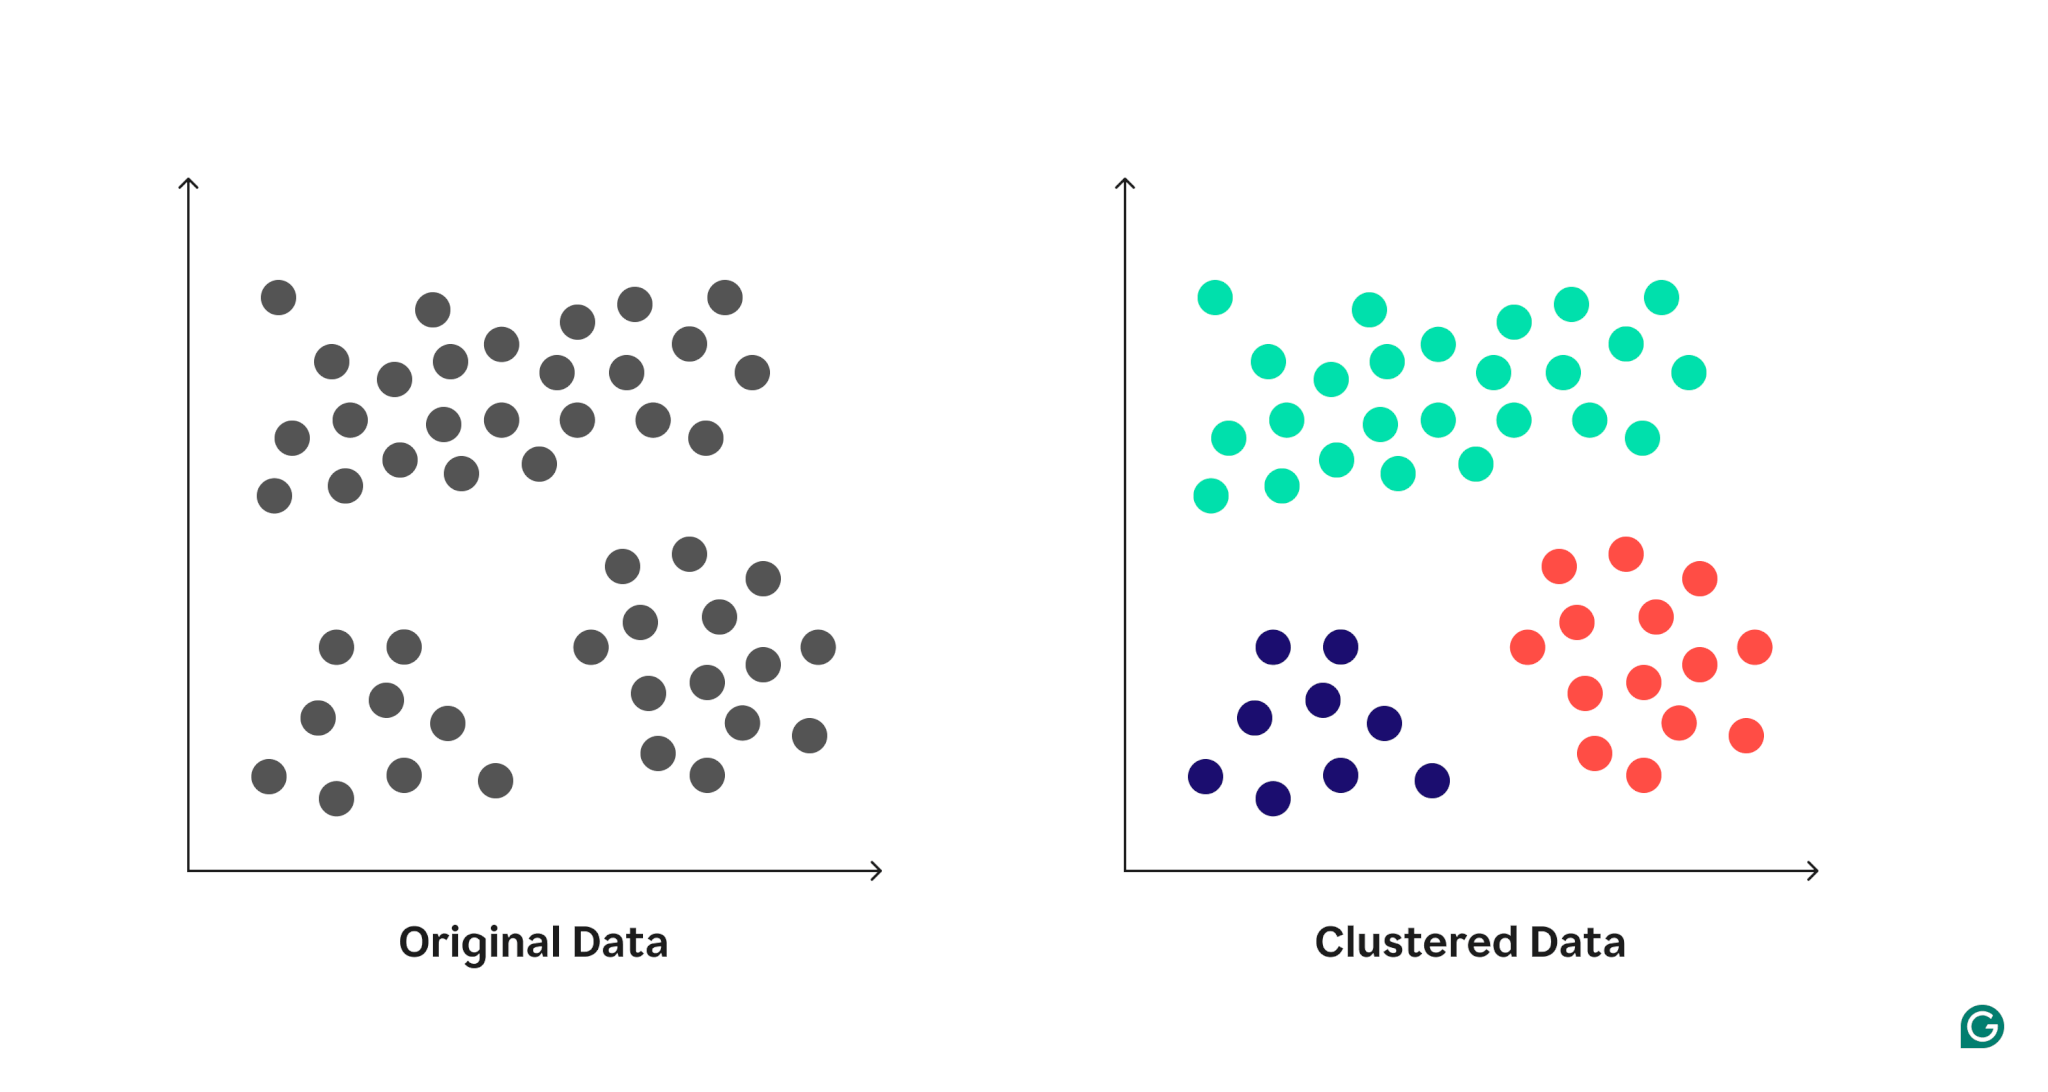
\includegraphics[width=0.9\textwidth]{Figures/Clustering_Data.png}
  \caption[Illustration of spatial data clustering]{Illustration of clustering of data points based on spatial proximity. Source: \url{https://www.grammarly.com/blog/ai/what-is-clustering/}}
  \label{fig:latlong}
\end{figure}


\subsection{Heat Map}
While clustering groups discrete points together, heat maps are used for data visualization to show relationship between variables and the density of data over a given area. The amount of data dictates a color gradient, leading to a higher concentration of data having a darker or warmer color than less concentrated areas. This leads to intuitive visualization of data for humans to parse, instantly highlighting "hotspots" of activity without needing to process individual data points. 
https://www.atlassian.com/data/charts/heatmap-complete-guide


\subsection{Scatter map}
A scatter map is a spatial adoption of a traditional scatter plot. Wherein a standard scatter plot is used to show correlation between variables on an abstract  x,y coordinate plane using statistical methods, a scatter map preforms this plotting using geographic coordinates. Each point of data is plotted using logitude as the X-axis and latitude as the Y-axis. This gives the user precise visualization of individual entities or incidents on a geographic map once a user zooms past the aggregated clustering layers.
https://www.atlassian.com/data/charts/what-is-a-scatter-plot

\section{Web Map}
Web maps are maps created for geographic visualization on the internet. They are a modern tool that allows users to have interactable maps on websites that are easy to use and insightful for what data is shown. Web maps are constructed by having a "basemap", which is the first layer showing the map itself without specific data. On top of the basemap, additional operational layers are added. This can be data points of incidents happening in a geographic area, charting of train tracks in a country, and much more that is defined by the needs of the user. 
https://www.mapbox.com/insights/web-maps


\subsection{vector tiles}
Vector tiles are the current standard utilized by most web map providers. Instead of the static PNG images that were used in the past, vector tiles save geographic data in a mathematical vector format. They allow for significantly more styling and customization than image-based formats, and have led to smoother, pixel-free zooming. However, because the browser must render the map geometry mathematically whenever the user zooms, this smoother usage comes at the cost of more processing power needed on the client's device.
https://docs.mapbox.com/data/tilesets/guides/vector-tiles-introduction/

\subsection{MapLibre}

\section{API}
In modern software architecture, an Application Programming Interface (API) is a crucial tool that allows communication between distinct software systems. In geographic applications, API's decouple the frontend web map from the from the backend database. So when a user interacts with the map, the frontend request specific subsets of data from the API, which returns the geographic coordinates in  a lightweight format such as JSON or GeoJSON.
https://aws.amazon.com/what-is/api/

\section{hardware acceleration}
Hardware acceleration is a method to get increased performance in computing tasks, which include rendering graphics and vector tiles in browsers. Hardware acceleration works by offloading tasks that are normally done by the CPU(Central Processing Unit) to other hardware in the computer like the GPU(Graphics Processing Unit). The GPU has massively more parallel processing capability than the CPU, significantly speeding up such computations for tasks that require it.
https://www.sciencedirect.com/topics/computer-science/hardware-acceleration

\subsection{WebGL}
In web enviorments, this hardware acceleration is achived via WebGL (Web Graphics Library).
\url{https://developer.mozilla.org/en-US/docs/Web/API/WebGL_API}


\section{Software principles}
To ensure that the software developed for this project remains scalable, maintainable, and robust, several core software engineering principles were adhered to. 

\subsection{Cohesion and Coupling}

\subsection{Testing}
lorem ipsum
lorem ipsum
lorem ipsum

\section{Agile Development}
This project was managed using Agile development principles. The Agile work flow prioritize adaptability, iterative progress, and continuous delivery. Which makes them ideal for software projects where technical requirements may evolve.
\subsection{Scrum and Issue Tracking}
lorem ipsum
lorem ipsum
lorem ipsum

%equations, bib. \\
%\section{Sprint/Scrum}
% Might make sprint its own section
\end{comment}
\begin{comment}
\section{Equations}

A simple equation can be included as: \\

\begin{equation}
        r = 2\pi^{2}
        \label{eqn:simple_eqn}
\end{equation} \\


\noindent The text below shows an example of how to align equations on the equal sign, with only one reference for both. This may be useful for when they are linked and are actually only one equation but splitting them up makes it more readable. \\

\begin{equation}
\begin{aligned}
        a &= \sin^{2}(\Delta\phi/2) + \cos(\phi_{1})\cdot\cos(\phi_{2})\cdot\sin^{2}(\Delta\lambda/2)\\
        d &= 2R\cdot\arcsin(\sqrt{a})
\end{aligned}
\label{eqn:haversine}
\end{equation} \\

\noindent The whole equation can be referenced as "equation \eqref{eqn:haversine}", here showing the Haversine formula. One may also align sub-equations such that they are numbered the same but have a letter differentiating them as shown below. This can be used when they are linked, but you will need to reference both individual parts.

\begin{subequations}
\begin{align}
    SSD 
        & \quad = \sum_{i=1}^{n} (\vec{x_{i}}-\vec{\mu_{q}})^{2} \label{eq:ssd}\\[15pt] %creates more space between the sub-equations
    SSE 
        & \quad = \sum_{q=1}^{k} \delta_{rq} SSD \label{eq:sse}
\end{align}
\label{eqn:subeqn}
\end{subequations} \\

\noindent These equations can be refrenced by their spesific sub-equation as "equation \eqref{eq:ssd}", or by the whole group as "equations \eqref{eqn:subeqn}". The "double backslashes" in the .tex creates line spaces and gives more room around the equations and paragraphs. Use them as you think feels right. 



\section{Tables and footnotes}

Here is an example of both a regular table with data and a table with split headers, for scientific usage. Do not use horizontal/vertical rulers between the data, or encase the table with rulers. \\

\begin{table}[ht!]
\centering
    \begin{tabular}{ m{3cm} m{2.5cm} m{2.5cm} m{2.5cm} m{2cm} } 
    \toprule
    \toprule
    \textbf{Statistic} & \textbf{Velocity} & \textbf{Altitude} & \textbf{1/Angle} & \textbf{Temp.} \\
    \midrule
    Mean    & 122.68    & 240.98   & 93.75     & 13.95 \\[1.3ex]
    Std     & 224.51    & 145.88   & 60.39     & 4.44  \\[1.3ex]
    Q1      & 28.00     & 111.60   & 34.15     & 10.60 \\[1.3ex]
    Median  & 63.00     & 223.20   & 99.59     & 13.30 \\[1.3ex]
    Q3      & 137.00    & 359.10   & 151.99    & 16.70 \\[1.3ex]
    Min     & 0.00      & 1.00     & 0.00      & 3.30  \\[1.3ex]
    Max     & 14519.00  & 616.70   & 180.00    & 32.10 \\[1.3ex]
    \bottomrule
    \bottomrule
    \end{tabular}
% the square brackets after \caption gives the table a proper title in the list of tables, instead of just inserting the beginning of the table caption
\caption[Dynamic feature statistics with outliers]{Table of dynamic feature statistics where outliers are included, for all data points. Velocity is given in \textit{m/h}, the altitude in \textit{mamsl}, the inverse trajectory angle in 1/degrees, and temperature in degrees Celsius.}
\label{table:stat_fliers}
\end{table}


\begin{table}[ht!]
\centering
    \begin{tabular}{ m{3cm} m{5cm} m{3cm} } 
    \toprule
    \toprule
    \textbf{Area 1} & \textbf{Start date} & \textbf{End date} \\
    \midrule
    2018    & 03.06    & 29.06                       \\[1.3ex]
    2019    & 03.06    & 03.07 or 31.08\footnotemark \\[1.3ex]
    2020    & 03.06    & 05.09                       \\[1.3ex]
    \midrule
    \textbf{Area 2} & \textbf{Start date (farm 1/2)} & \textbf{End date} \\
    \midrule
    2012    & 09.06            & 07.09               \\[1.3ex]
    2013    & 23.06 / 15.06    & 25.08               \\[1.3ex]
    2014    & 05.06 / 25.06    & 10.09               \\[1.3ex]
    2015    & 13.06 / 03.07    & 06.09               \\[1.3ex]
    2016    & 17.06            & 22.07               \\[1.3ex]
    \bottomrule
    \bottomrule
    \end{tabular}
\caption[Selected time ranges for all data]{Selected time ranges for the data in all areas and all years.}
\label{table:time_ranges}
\end{table}

\footnotetext{A footnote explaining something.}



\section{A single figure}

Figure \ref{fig:latlong} is included as an example. The square brackets before the caption description contains the title of the figure, which is what will be written in the list of figures. This should be short and concise. The same layout applies to tables and other floats. Remember to change the title as well as the caption if you are copying these examples. In the list of figures and tables all the different floats will be grouped together by chapter. Remember to always reference all your figures and tables in the text at least once.

\begin{figure}[H]
  \centering
  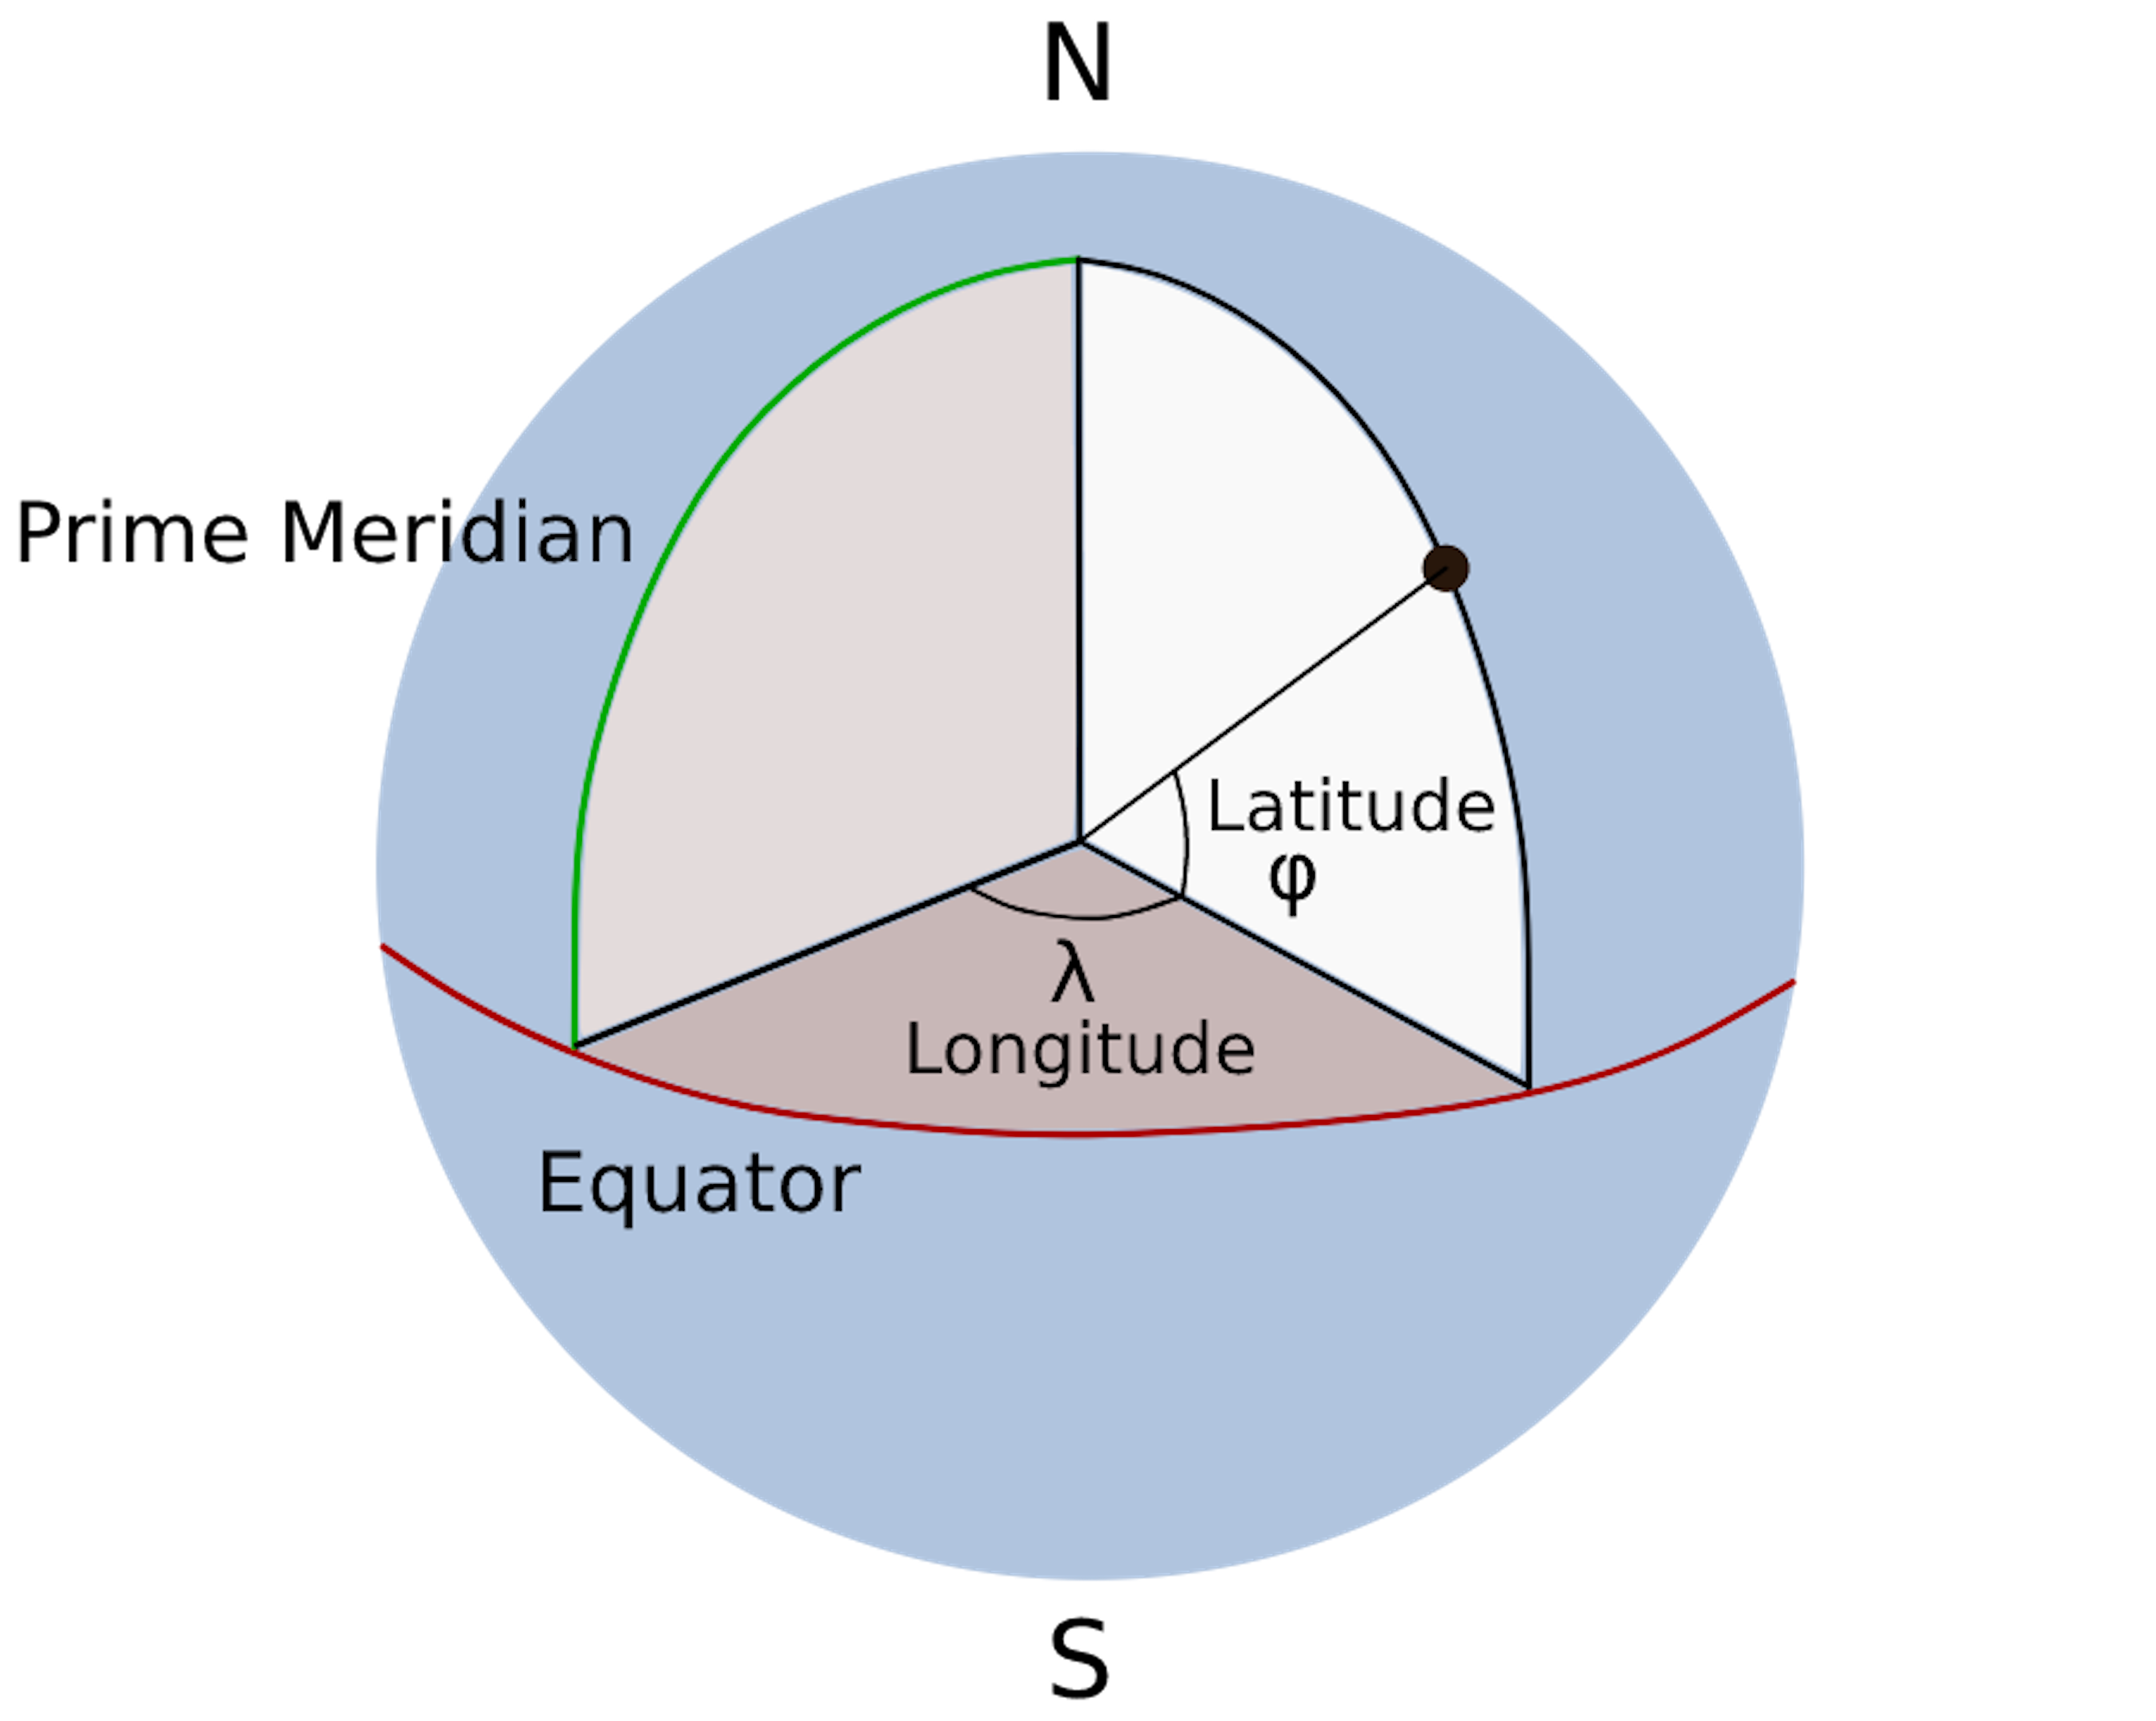
\includegraphics[width=0.9\textwidth]{Figures/latlong.png}
  \caption[Illustration of latitude and longitude]{Illustration of the earth, and how latitudes and longitudes are calculated with respect to the equator and the prime meridian.}
  \label{fig:latlong}
\end{figure}


\section{Citations}

Here are some examples on how to reference a source (where none is relevant to the text but just for illustration purposes only). One may cite a single reference by calling \cite{wolves_of_mount_mckinley}, or several in the same bracket by calling \cite{machine_learning, clustering_impossibility} when they are all related to the same statement. There are many different styles on how to cite, and how the layout and order of your citation style is presented. This is my favorite, as I find it neat and tidy \cite{sheep}. It will show up in order of appearance in the references section.
\end{comment}
\cleardoublepage


\chapter{Methods}
% This chapter describes the methodology, tools, and implementation choices
% used during the development of the AIS anomaly visualisation prototype.

\textit{This chapter outlines the development process, tools and frameworks used, system architecture, and testing strategies employed throughout the project.}

%=====================================================================
% 3.1  Development Methodology
%=====================================================================
\section{Development Methodology}

% FOCUS: Describe HOW you organised the project. Sprint structure,
% meeting routines, roles, and task tracking.
% Mirror the chess thesis Section 3.3 for level of detail.

%The team used an Agile approach with the Scrum framework to organise the project. Work was divided into sprints of one to two weeks, where sprint length was adjusted depending on workload from other courses.
% Unsure about what Arne should be called. Since he controls everything so just put him down as supervising lecturer.
\subsection{Scrum Framework}
The Scrum framework, described in Section 2.X, was adopted to structure the development process. The framework was introduced by the supervising lecturer, who provided pre-filled sprint templates and documentation to support its application for groups. This lowered the time investment of adopting the system and methodology, while ensuring that sprint artefacts such as the backlog and retrospectives were maintained throughout the project. Scrum was also well suited given the projects biweekly meetings with the supervisor and the customer at Kystverket. Each sprint would ensure that further development in the project could be presented and discussed, allowing scope adjustments to be made based based on the feedback. Should technical issues occur, such as limitations or issues with the AIS dataset or uncertainty around feasibility or scope for specific visualisation features. Then the iterative structure allows focus on the backlog until discussions about scope or features are had with the customer at Kystverket rather than following a fixed plan.

\subsection{Daily Stand-Ups}
Daily stand-up meetings were established as a core part of the sprint work flow, in line with the Scrum practices described in Section 2.X. The primary purpose of the stand-ups is to maintain accountability between team members and to further facilitate collaborative problem-solving between team members depending on problems blocking further development. In a two-person team, the risk of one member being stuck on a problem without the other member being aware is likely. Therefore by utilizing a daily meeting it allows such issues to be discussed early and not let it stop further project development. They can also be utilized as a daily forced break for the team. Sustained work without regular breaks is not equated to consistent productivity, while also being a way to quickly discuss a problem for further collaborative work after the stand-up meeting.


%Every day the team had a stand-up meeting at 12:00 where members discussed issues they had run into, what they were working on, and what to focus on next. However a lot of days we had multiple daily stand ups to clear our head and keep motivation high.

The project spanned from January 2026, with delivery on the 20th of May. 

The project was initially started by a team of three members. However one member withdrew from the project early in the semester due to personal reasons. The remaining two members, continued development and divided the responsibility between them. One member served as Scrum Master and maintained the sprint documentation, while the other handled meeting notes. All other responsibilities including development, testing, and design were shared equally.
% TODO: Add about issues with workload and how we handled it.

Biweekly meetings were held with the supervisor to review academic progress and get guidance. We also mostly had biweekly meetings with the customer at Kystverket which were arranged to present progress, get feedback, and clarify scope.
% TODO: Maybe talk about how they were busy some times also wondering how to word kystverket.

\subsection{Task Management}

Task tracking was handled using GitHub Projects, which provided a shared Kanban-style board across the team's three repositories: one for the frontend, one for the backend, and one for administrative documents like meeting notes and sprint documentation. Issues were created and tracked through workflow stages to maintain workload transparency and motivation.
% TODO: Maybe add link and theory to theory chapter
% https://docs.github.com/en/issues/planning-and-tracking-with-projects/customizing-views-in-your-project/customizing-the-board-layout

%=====================================================================
% 3.2  Tools and Platforms
%=====================================================================
\section{Tools and Platforms}

\subsection{Development Tools}
\begin{itemize}
\item \textbf{Visual Studio Code:} Primary development environment used by all team members.
\item \textbf{Git \& GitHub:} Used for version control, branching, pull requests, and task management via GitHub Projects.
\item \textbf{Docker:} The backend was containerised using Docker to ensure a consistent and reproducible runtime environment.
\item \textbf{Swagger:} Used for API documentation and testing of backend endpoints.
\end{itemize}

\subsection{Design Tools}
\begin{itemize}
\item \textbf{Figma:} Used for designing wireframes and UI mockups for the web application.
\end{itemize}

\subsection{Communication Tools}
\begin{itemize}
\item \textbf{Discord:} Primary communication platform for team discussions, quick coordination, and informal meetings.
\item \textbf{Slack:} Used for communication with the customer (Kystverket), including asking technical questions and discussing issues.
\item \textbf{Outlook:} Used for planning meetings with Supervisor.
\end{itemize}

\subsection{AI Tools}
\begin{itemize}
\item \textbf{ChatGPT \& Gemini:} Primarily used for technical issues, understanding technologies, and spell checking. 
\end{itemize}

% TODO: Talk with other group member about their ai usage to make sure nothing is missing
% TODO: Add other tools


%=====================================================================
% 3.3  Technology Stack
%=====================================================================
\section{Technology Stack}

The technology stack was primarily decided by the customer's existing infrastructure. Since the prototype is intended to work with Kystverket's systems, using their technology choices ensures compatibility. It also allows the team to leverage the customer's expertise if questions arise, since this is a prototype using their techstack.

\subsection{Frontend}
\begin{itemize}
\item \textbf{React \& TypeScript:} Core frontend framework and language, chosen as a requirement from the customer.
\item \textbf{MapLibre GL JS:} Mapping engine used for rendering interactive, high-performance maps with WebGL acceleration.
%\item \textbf{Vite:} 
% TODO: Go over as a group to make sure no libraries or dependencies are missing.

\end{itemize}

\subsection{Backend}
\begin{itemize}
\item \textbf{PostgreSQL:} The database storing the AIS anomaly test data, provided by the customer.
\item \textbf{Swagger:} API documentation is auto-generated using Swagger annotations in the Go source code. A Swagger UI endpoint is available for exploring and testing the API.
\item \textbf{Docker:} Used for containerising the backend services.
% TODO: Mention other things used in the backend making sure nothing is missing.
\end{itemize}

The backend was originally provided by Kystverket as a working codebase pre-populated with test data, since actual AIS anomaly data is confidential. The team forked this repository and updated it throughout the project. The most notable addition was a master query endpoint described in Section 3.4.1
% TODO: Describe the test dataset briefly (rough size, time range, types of anomalies if known).

%=====================================================================
% 3.4  System Architecture
%=====================================================================
\section{System Architecture}

% FOCUS: Describe how the pieces fit together. Include a diagram if possible.
% The chess thesis has sequence diagrams, class diagrams, package diagrams —
% you should have at least one architecture diagram here.

% TODO: Add a figure showing the overall system architecture.
% A simple box diagram: Database <-> Backend (Go/Docker) <-> REST API <-> Frontend (React/MapLibre)

The system follows a client-server architecture. The backend is written in Go and runs inside a Docker container that exposes a REST API. Swagger is used for API documentation. The frontend is built with React and TypeScript and retrieves the data it needs through API calls to the backend.

\subsection{Backend and Data Flow}

The backend infrastructure and test database were provided by the customer, pre-populated with test data since actual AIS anomaly data is confidential. The team's main contribution to the backend was a master query endpoint. This endpoint accepts all filter parameters (anomaly type, mmsi, and time range.) and returns only the matching data. Instead of getting all the anomaly groups and filtering on the frontend, all variables get sent to the backend which queries the data again. This was done since keeping old data and filtering client-side was slow and inefficient.

% TODO: Maybe include how data is returned and used? Geojson and such

\subsection{Frontend Architecture}
The frontend architecture follows a client-driven data flow where data is retrieved from the backend through REST API calls using Axios. The received data is stored in React state as a geoJSON featureCollection, which is passed to individual Deck.gl layers responsible for rendering the visualisations. This is done after a map instance is created through a map container class, using maplibre. deck.gl is subsequently used for rendering data points overlaid visually on the map. Interactivity is handled through React components, where state changes control filtering and updating of the rendered layers. Individual Deck.gl layers also implement click event handlers, which update application state and trigger the rendering of additional information components or different visualization layers. 

% TODO: Describe the React component structure at a high level.
% - How is routing handled?
% - What are the main pages/views? (Map view, filter panel, detail cards, etc.)
% - How does state management work for filters and map state?

%=====================================================================
% 3.5  Visualisation Implementation
%=====================================================================
\section{Visualisation Implementation}

% FOCUS: This is your core contribution — give it proper space.
% Describe HOW you implemented each visualisation technique from your Theory chapter.

\subsection{Map Setup and Rendering}

The base map is implemented using MapLibre GL JS, as the engine for rendering the map. based on a vector tile set from openFreeMap  \url{https://tiles.openfreemap.org}. \label{sec:vector tiles} The tile set chosen was bright in color. Deck.gl was chosen for rendering data points on the map, with points being overlaid on top of the base map



% TODO: Describe the base map setup:
% - What vector tile source did you use? (customer-provided? OpenMapTiles? Maptiler?)
% - Any custom map styles?
% - Initial map center, zoom level, bounds?

\subsection{Clustering}


As mentioned in Section \ref{sec:supercluster}, Supercluster.js is used for calculating clusters based on zoom level and the current map bounds. Supercluster calculates clusters based on the base dataset acquired from the API, calculating all clusters on application load. Map interactions such as zooming and dragging result in clusters being retrieved for the current zoom level and map bounds. The clustering data itself is used with deck.gl,Section \ref{sec:deckgl}. Visualization through deck.gl is accomplished through creating a custom layer, consisting of a label-layer, whose purpose is to be a point counter for the amount of anomalies inside the cluster, this is put over, a scatterplot-layer. section \ref{sec:scattermap}, which combines to create the clustering layer.This layer is re-rendered whenever the clustering output changes due to updates in zoom level or map bounds. Furthermore does clustering visualization have dynamics sizing based on amount of anomalies inside a cluster, leading to clusters being scaled proportional to their anomaly count. 

% TODO: Add technical details:
% - What clustering radius/parameters did you use?
% - How are cluster colours determined (step expressions? interpolation?)
% - Any custom cluster styling?
% - add figure

\subsection{Heat Map}
A heat map layer was implemented for visualization of the full dataset. \ref{sec:heatmap}. deck.gl was used for heat map visualization, where the library provided the methods to create the heat map, with the data provided being the base API data of the full dataset. 
% TODO: Describe the MapLibre heat map layer configuration:
% - What colour ramp did you use?
% - How does the weight/intensity scale with zoom?
% - Any specific property used for weighting (e.g. anomaly severity)?


\subsection{Anomaly Group Layer}
The anomaly group layer, is a visualization layer that gives a detailed representation of a single anomaly group, section \ref{sec:anomalies and anomaly groups}. The anomaly group visualization layer is created through a custom deck.gl layer. This layer consists of a signal strength layer, using data from the individual anomalies inside the group, that are connected to a satellite or base station with a signal strength number value, normalized between 0 and 1. The signal strength layer adds lines from the source anomaly, to the receiving base station and or satellite, indicating the strength of received AIS-message.   





\subsection{Frontend Components}


\subsection{Scope and Feature Prioritisation}

The project scope was decided through ongoing discussions with the customer. Hexagonal binning was initially identified as a desired feature in the project brief. However due to time constraints it was not implemented in the final prototype. The team prioritised clustering, heat maps, and the filter system based on customer feedback since these provided the most immediate analytical value. 
% TODO: Include what we cut / didnt focus on
% NOTE TO SELF: Your Introduction (Section 1.2 Objective) lists hexagonal binning
% and advanced temporal analysis as goals. Since hex binning was not implemented
% and temporal analysis is limited to time-range filtering, you should either:
%   (a) soften the Introduction wording (e.g. "investigate" instead of "implement"), or
%   (b) address the gap explicitly in Discussion (recommended — explain the
%       scoping decision made with the customer).


\subsection{Filter System}



\subsection{Temporal Filtering}



\subsection{Interactive Features}


%=====================================================================
% 3.6  Design Process
%=====================================================================
\section{Design Process}

% FOCUS: Wireframes, UI/UX decisions, user feedback.

\subsection{Wireframes and UI Design}


\subsection{User Feedback}


%=====================================================================
% 3.7  Testing
%=====================================================================
\section{Testing}

% FOCUS: What you tested, how, and why certain approaches were chosen.

\subsection{Backend API Testing}


\subsection{Frontend Testing}


\subsection{Manual and Performance Testing}

%=====================================================================
% End of Methods chapter
%=====================================================================

\cleardoublepage


\chapter{Results}
%=====================================================================
% 4. RESULTS — SECTION ORDER (mirrors Method 3.1–3.8):
%   4.1 Project Overview        (brief intro, no Method counterpart)
%   4.2 Project Management      <- Method 3.1
%   4.3 System Architecture     <- Method 3.2
%   4.4 Frontend                <- Method 3.3
%   4.5 Backend and Data Handling <- Method 3.4
%   4.6 Visualization Results   <- Method 3.5
%   4.7 Filter and Interaction  <- Method 3.6
%   4.8 Testing and Performance <- Method 3.7
%   4.9 Customer Feedback       <- Method 3.8
%   4.10 Project Outcome
% Outstanding work is marked inline with "% SUGGESTION:" comments (content you write yourself).
%=====================================================================
\textit{This chapter outlines the results of the project, explaining the functionality and design of the completed project.}
% Might change it to not have this section and make it all into intro.
% SUGGESTION (4.1 overview — you write any new prose): the intro paragraph below reads fine and
% already lists the delivered features. Keep it short and factual. Any code-quality evaluation
% belongs in Discussion, not here.
%TODO In relation to tool choice might mention it more in method or result to be clearer over why we chose them.

This chapter presents the resulting application, a locally hosted visualization tool for AIS anomalies and anomaly groups. The system implements clustering, heat map, base station, anomaly group, and individual anomaly visualization layers, supported by a filtering system and interactive features. The technology stack was partly guided by the customer, with React and the map provider specified, while remaining tool choices were made by the group. The following sections describe the delivered system, organized in the same order as the Method chapter: project management, system architecture, frontend, backend and data handling, visualization, filtering and interaction, testing and performance, customer feedback, and project outcome.

\newpage
\section{Project Management}
\label{sec:results_project_management}

The project followed the Scrum-based process described in Section~\ref{sec:dev_methodology}, divided into approximately 16 weekly sprints, with occasional two-week exceptions over the project period. Each sprint included a sprint planning session, daily synchronization meetings, and a retrospective. Bi-weekly meetings were held with both the supervisor and the customer at Kystverket, though scheduling occasionally extended the interval to three weeks. At the end of the project, the GitHub Projects contained 106 completed issues across the frontend, backend and administrative repositories.

During the project team roles were maintained with expections made in case of illness if work needed to be done in that role, however it was mostly delayed until the person could handle it.
% SUGGESTION (4.2, optional content — you write it): Method 3.1 has seven subsections but this
% result mirrors only Scrum. If you want symmetry, add ONE factual sentence on team roles (who
% owned what) and ONE on how the 106 issues split across the three boards. Keep it factual — no
% judgement on whether Scrum worked (that belongs in Discussion / Project Execution).


\section{System Architecture}
\label{sec:results_system_architecture}

The final system architecture, resulting from the design described in Section~\ref{sec:system_architecture}, consists of a React frontend communicating with a backend REST API. The frontend is responsible for rendering visualization layers and handling user interaction, while the backend provides GeoJSON-formatted anomaly data and database generation. The architecture separates visualization, filtering, and data retrieval into different parts. The following diagrams illustrate the system's structure, data flow and user interaction.


\subsection{Use Case Diagram}

\begin{figure}[H]
    \centering
    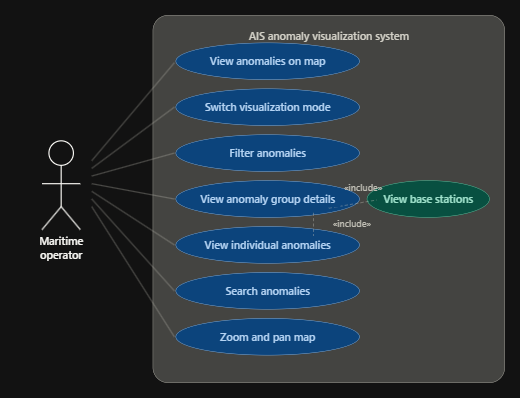
\includegraphics[width=0.95\textwidth,height=0.7\textheight,keepaspectratio]{Figures/Use_Case_Diagram.png}
    \caption[Use Case Diagram]{Use case diagram showing the expected interactions between a maritime operator and the system's core features}
    \label{fig:Use_Case_image}
\end{figure}

The use case diagram in Figure~\ref{fig:Use_Case_image} illustrates the expected user experience for a maritime operator. It showcases the core capabilities delivered by the system, allowing an operator to view anomalies, switch between different visualization layers, and access specific information regarding individual anomalies and anomaly groups.

\subsection{Package Diagram}

% SUGGESTION: replace with an updated package-diagram image if the directory structure changed.
\begin{figure}[H]
    \centering
    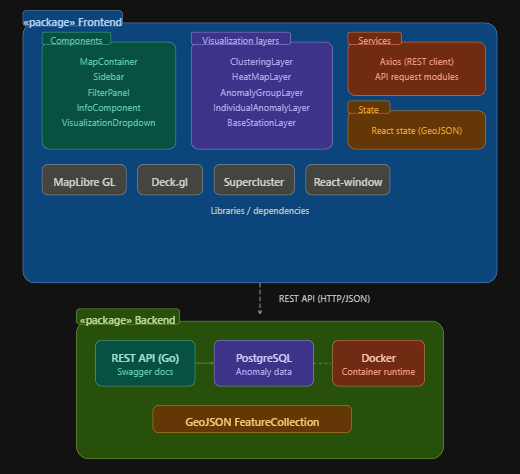
\includegraphics[width=0.95\textwidth,height=0.7\textheight,keepaspectratio]{Figures/Package_Diagram.png}
    \caption[Package Diagram]{Package diagram showing the modular directory structure of the frontend repository}
    \label{fig:Package_Diagram_image}
\end{figure}

The package diagram in Figure~\ref{fig:Package_Diagram_image} outlines the modular directory structure used in the frontend repository. Files are put into folders related to their function, such as components being isolated within a dedicated component folder, with necessary subfolders. This aligns with standard React component patterns as described in ~\ref{sec:react_theory}.

%TODO might need to add more theory to be able to better explain directory and patterns. also update the diagram to include all packages.
%, ensuring the codebase remains modular and easily navigable.
% SUGGESTION (relocate evaluation — your call): the clause "ensuring the codebase remains modular and
% easily navigable" is an assessment, not an observation of the diagram. Consider moving that
% judgement to Discussion (Technical Solution / Code Quality) and keeping only the structural fact
% here. Also verify you have a Theory reference for React package structure if you want to cite it.


\subsection{Sequence Diagram (Data Flow)}

\begin{figure}[H]
    \centering
    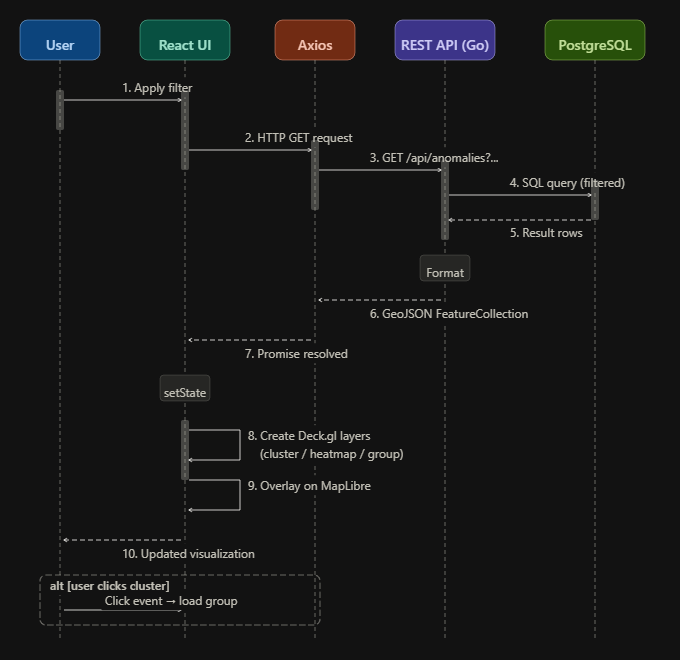
\includegraphics[width=0.95\textwidth,height=0.7\textheight,keepaspectratio]{Figures/Sequence_Diagram.png}
    \caption[Sequence Diagram]{Sequence diagram illustrating the data flow from a user filter action to an updated visualization layer}
    \label{fig:Sequence_Diagram_image}
\end{figure}

The sequence diagram in Figure~\ref{fig:Sequence_Diagram_image} maps the data flow from user interaction to visual state change. As illustrated in the image, if a user requests to apply a filter, an HTTP GET request is sent to an endpoint, which then queries the database. This then returns a GeoJSON FeatureCollection as a promise, and is then asynchronously accessed through React. This then creates the Deck.gl layer requested, and overlays it on the map, leading to an updated visualization for the end user.

\subsection{MapLibre}
% MOVED here from Visualization Results (4.6): MapLibre is architecture/runtime behaviour, mirroring
% its place under System Architecture in Method 3.2, not a visualization result.
MapLibre initializes itself upon application boot, in a bright style used for readability for users. After its initialization, it is responsible for interaction, in dragging and zooming the map. Interaction leads to states being updated that other parts of the program can use, such as clusters being updated through zooming, and map location. Visualization functionality is something MapLibre has, being able to natively visualize scatterplots and other layers. 
%TODO Start mentioning more about rational for choosing diffrent tools in method outside of them being suggested talking maybe about testing them before choosing.
%This was not chosen as a valid approach of visualization in the project, due to the high amount of data required to be visualized, which Deck.gl is specialized for.
% SUGGESTION (your call): the last sentence (why MapLibre was not used for visualization) is design
% rationale that may fit better in Method 3.2 (System Architecture / MapLibre) than in Results.

\section{Frontend}
\label{sec:results_frontend}
The resulting frontend of the project was created following the method in Section~\ref{sec:design_process}. Figure~\ref{fig:frontend_result_image} shows the finished frontend.

\begin{figure}[H]
    \centering
    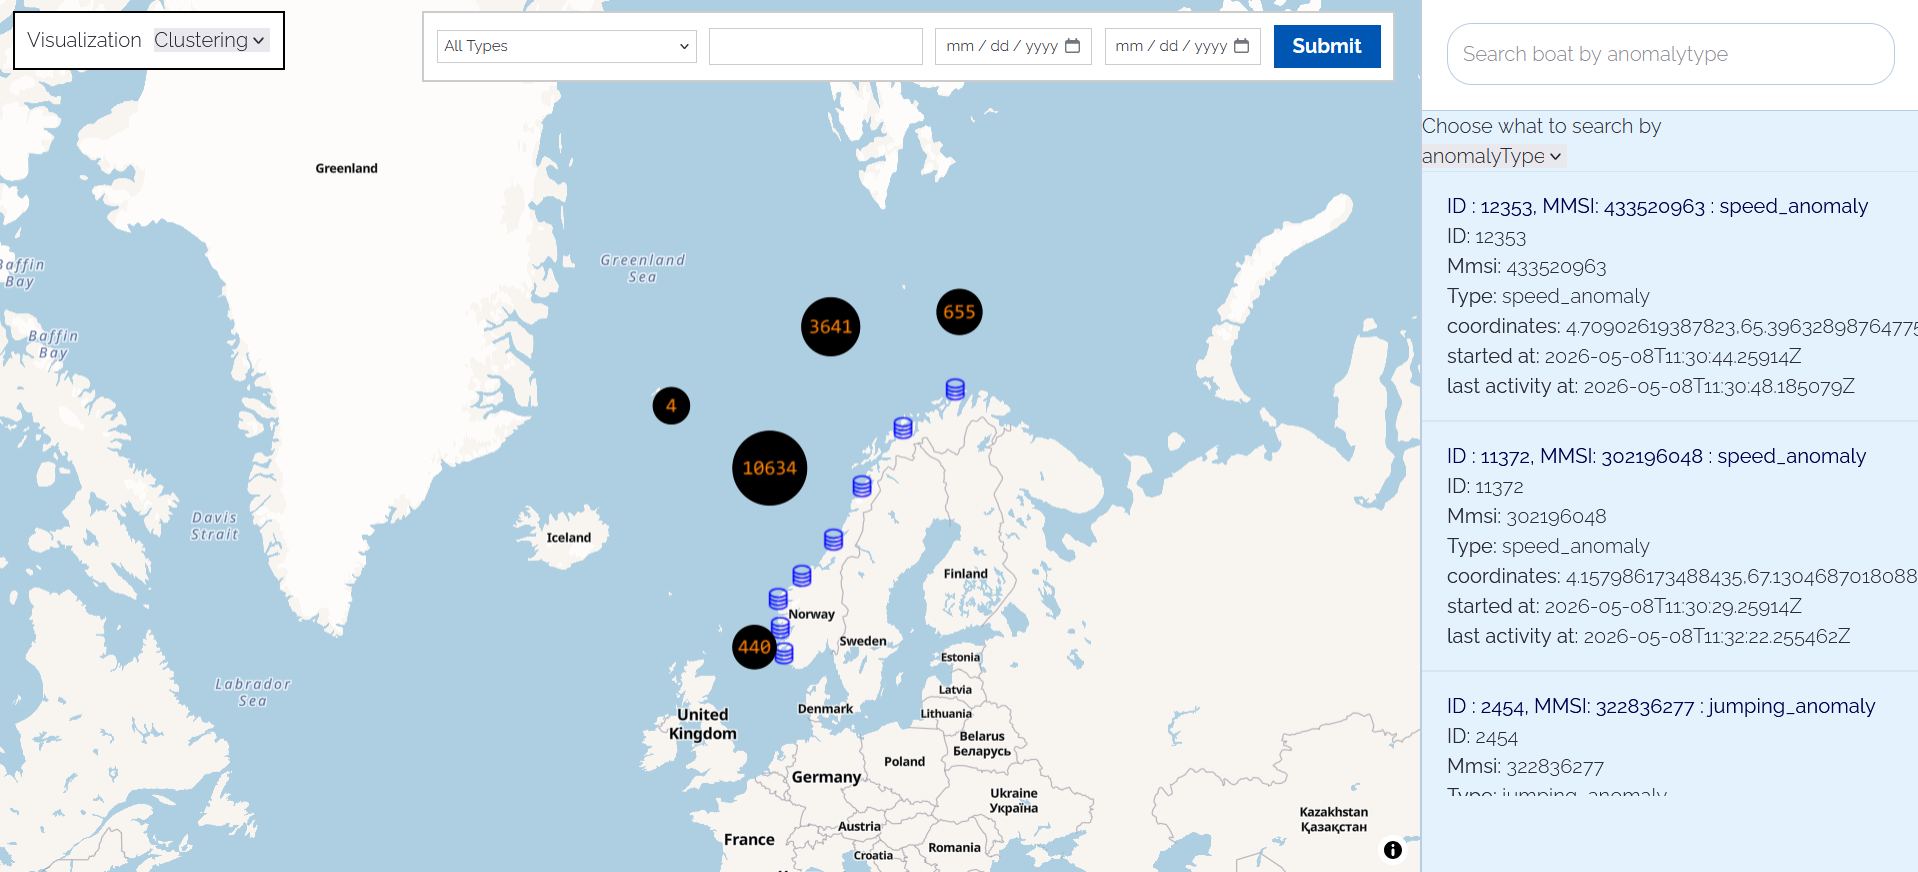
\includegraphics[width=0.95\textwidth,height=0.7\textheight,keepaspectratio]{Figures/full_application_image.png}
    \caption[Frontend application]{The completed single-page application showing the map view with visualization overlay, sidebar, and filter component}
    \label{fig:frontend_result_image}
\end{figure}

A singular page was created for the application, being the only page needed for all functionality. As shown in Figure~\ref{fig:frontend_result_image}, the user interface is made up of multiple parts. The base map takes up the center of the application, with visualization overlaid on top of the map.

Components such as a sidebar on the top right contain the entire dataset, allowing for searching of anomalies based on type or MMSI. 
A visualization dropdown menu allows switching between the two main visualization modes. 
On the top middle of the page is a filtering component, allowing users to change the displayed dataset by filtering on anomaly type, date range, and MMSI.
% SUGGESTION (4.4, wireframe link — you write the sentence(s)): add a link from the final UI back to
% the wireframes in Method 3.3. State whether the layout follows each wireframe (main page, date
% picker, filter) or diverged — e.g. the filter being moved to the top middle after customer
% feedback. Divergence-with-reason scores higher than "it matches", because it shows the design
% process fed real decisions.
%TODO add info since it wasa decided that the filter was moved to the top and after multiple visualization methods were added the top left has a permanent area for swapping betting clustering and heat maps. Also compared to the filter componenent it is wide to reduce clutter on the main page compared to the old filter in wireframe which had multiple fields for custom values as well as expandable lists for filtering. The final system became simpler with it only including type, mmsi and start and end date. While the sidebare stayed mostly the same however it now covers the whole right side. top to bottom. The ship info card stayed mostly the same with just a new button, which can show the anomalies in the group. Which was requested by the customer.

\section{Backend and Data Handling}
\label{sec:results_backend_and_data}
The backend, described in Section~\ref{sec:backend_and_data_flow_method}, was developed by the customer and provided as part of the project infrastructure. It exposes a REST API used by the frontend to retrieve anomaly data. Anomaly data is stored as a GeoJSON FeatureCollection, with each feature representing a single anomaly group.
\begin{figure}[H]
    \centering
    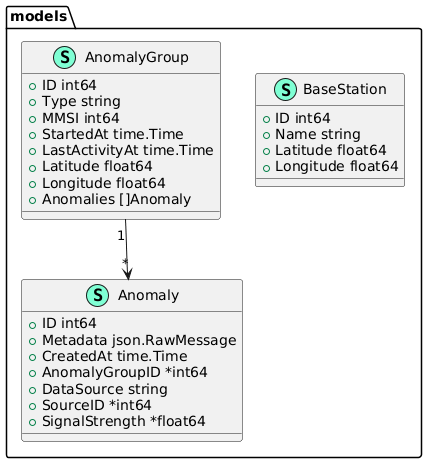
\includegraphics[width=0.54\textwidth,height=0.4\textheight,keepaspectratio]{Figures/db_models.png}
    \caption[Database model diagram]{Database model diagram showing the relationship between anomaly groups and individual anomalies}
    \label{fig:databse_model_diagram_image}
\end{figure}

\begin{figure}[H]
    \centering
    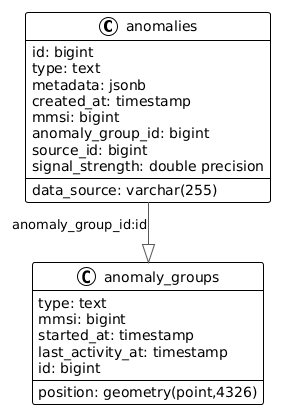
\includegraphics[width=0.54\textwidth,height=0.4\textheight,keepaspectratio]{Figures/db_result.png}
    \caption[Database schema]{Database schema showing table structure, field definitions, and data types}
    \label{fig:database_schema_image}
\end{figure}

Figures~\ref{fig:databse_model_diagram_image} and~\ref{fig:database_schema_image} show the backend database structure. An anomaly group contains anomalies, where the anomaly group itself has the start time and last activity time, sourced from the first instance of an anomaly being created in a group. Anomalies themselves have signal strength and their own data, with the group containing general data related to the group such as the general area of the anomalies, represented as location. 

The anomalies and anomaly groups are generated by the Docker backend, with the amount of anomalies set through a configuration file. Specific commands to generate anomalies and build the database are used, leading to a database filled with an amount of points set by the developer. The Docker backend running allows for the frontend to send requests to API endpoints to request data, while the frontend itself runs through localhost.

\subsection{GeoJSON Data Structure}

The final GeoJSON structure is shown in Figure~\ref{fig:geoJSON-result_image}.
\begin{figure}[H]
    \centering
    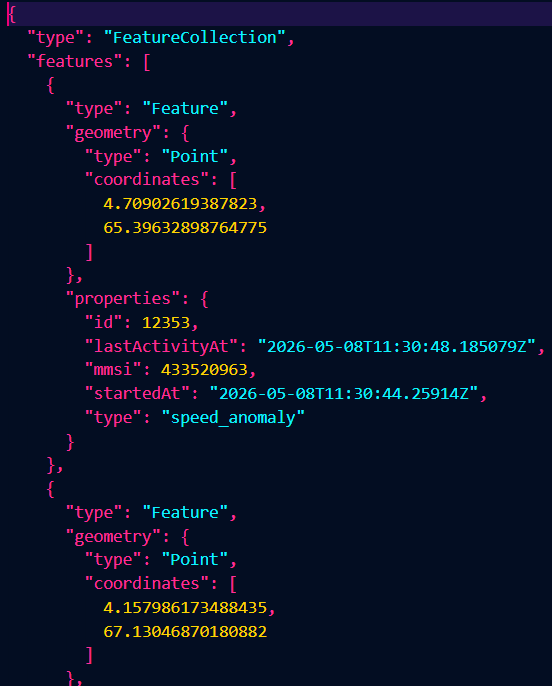
\includegraphics[width=0.54\textwidth,height=0.4\textheight,keepaspectratio]{Figures/geoJSON-result.png}
    \caption[GeoJSON FeatureCollection structure]{Example GeoJSON FeatureCollection returned by the backend API, with anomaly groups as individual features}
    \label{fig:geoJSON-result_image}
\end{figure}
Anomaly data is completely integrated in a FeatureCollection, with the individual features being anomaly groups. These features are individually processed in the frontend, as a dataset, through Deck.gl.

\subsection{Backend Query and Response Behaviour}
Figure~\ref{fig:swagger-result_image} showcases an API endpoint, created as a master query allowing for filtered requests on all relevant variables.
% SUGGESTION (own-contribution — you write it): the master query is one of your strongest own
% contributions. Name the parameters it accepts (e.g. anomaly type, MMSI, time range) and what a
% typical response contains, and bridge to Method 3.4 (Section~\ref{sec:backend_and_data_flow_method}).
% Make the boundary explicit: backend infrastructure was the customer's, this endpoint was the group's.
%TODO anomaly type, MMSI, time range were all included in the master query, this was a contribution to backend infrastructure the customer provided. Creating a new endpoint which returns all the anomaly groups with those variables. which includes all anomalies which includes base stations and signal strength within. Unsure if i should mention all that.

\begin{figure}[H]
    \centering
    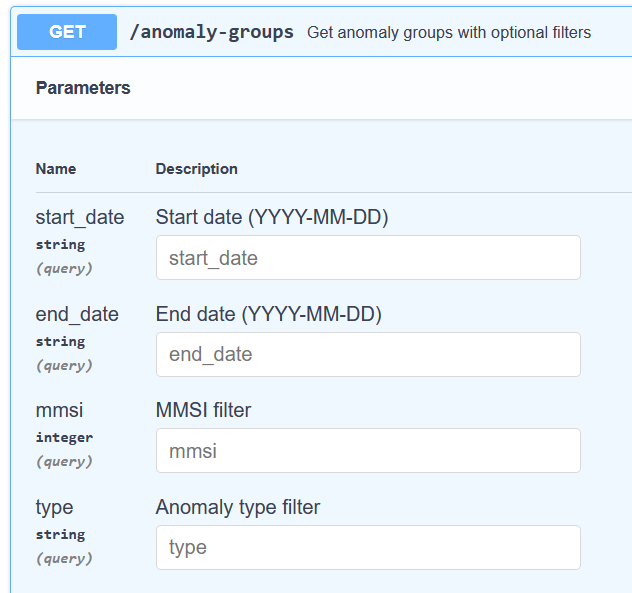
\includegraphics[width=0.54\textwidth,height=0.4\textheight,keepaspectratio]{Figures/swagger_api.png}
    \caption[Swagger API endpoint]{Swagger UI showing the master query endpoint with all available filter parameters}
    \label{fig:swagger-result_image}
\end{figure}
General endpoints for retrieving all anomaly data, as well as filtered datasets, are implemented. Requesting filtered data leads to the base dataset changing to contain the new data, while in other cases such as the sidebar having its own data variable to not change the main map data through search.

\section{Visualization Results}
\label{sec:results_visualization}
All visualization methods described in the Method chapter were implemented in the final system. The system includes clustering, heat map, base station, anomaly group, and individual anomaly visualization. Additional proposed features were not implemented.

\subsection{Clustering Visualization}
The clustering visualization was implemented as described in Section~\ref{sec:clustering_method}. The clustering approach uses Supercluster.js to calculate clusters through proximity based on radius and zoom level (Section~\ref{sec:supercluster}). This approach produces grouped anomaly points, with numeric labels indicating the number of anomalies in each cluster, as shown in Figure~\ref{fig:clustering_result_image}.
\begin{figure}[H]
    \centering
    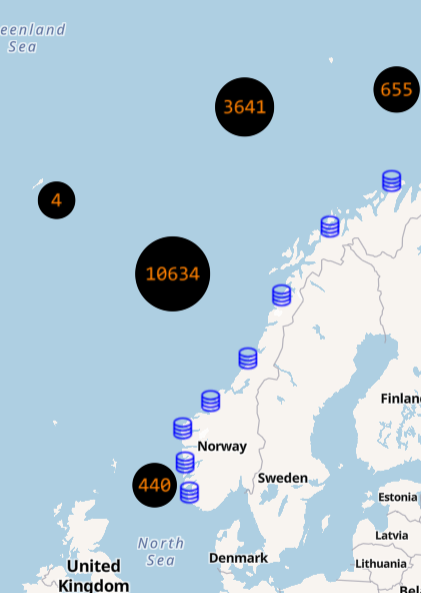
\includegraphics[width=0.4\textwidth,height=0.35\textheight,keepaspectratio]{Figures/clustering-result.png}
    \caption[Clustering visualization result]{Clustering visualization showing anomaly groups aggregated by proximity, with numeric labels indicating the group count per cluster}
    \label{fig:clustering_result_image}
\end{figure}
Clusters are calculated through the use of a radius that computes the amount of points inside a circle of a defined radius, in the case of the project being 40 pixels. Points inside the pixel radius are aggregated, and shown as a single point. A higher density of points in a cluster leads to that cluster being shown as larger on the map. Recalculation of clusters happens when zooming and dragging is done in the application, where clusters are divided into smaller parts due to points increasing in distance, moving outside of the defined radius.
% SUGGESTION (Method/Results bleed + figure-specific — your call): this paragraph re-derives the
% 40-pixel aggregation mechanism, which is really Method 3.5 content. Consider moving the mechanism to
% Method and replacing it here with what YOUR screenshot actually shows: which region, which zoom
% level, where the largest cluster sits and roughly how many anomalies it holds. The clustering
% performance effect is reported in Section~\ref{sec:effect_of_clustering_results}.
%TODO Use the image like suggested to show how it works now.


\subsection{Heat Map Visualization}
The system includes a heat map visualization layer. The heat map is implemented as in Section~\ref{sec:Heat_Map_method}. An example of the implemented heat map visualization is shown in Figure~\ref{fig:heatmap_result_image}.
\begin{figure}[H]
    \centering
    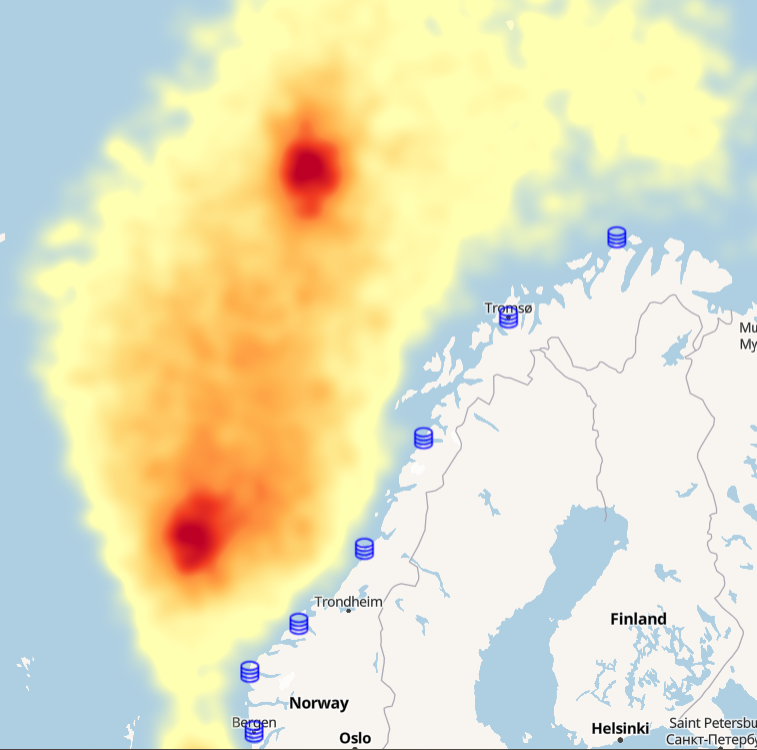
\includegraphics[width=0.54\textwidth,height=0.35\textheight,keepaspectratio]{Figures/heatmap-result.png}
    \caption[Heat map visualization result]{Heat map visualization showing anomaly density across the dataset, with warmer colors indicating higher concentrations}
    \label{fig:heatmap_result_image}
\end{figure}
Color is generated through calculating the sum of points inside a radius of 40 pixels, meaning points inside a circle are calculated as a sum, leading to higher density of points being weighted more \parencite{deckgl_official_site}. 
The resulting heat map layer allows for zoom and drag operations to change the heat map view dynamically, with zoomed in levels having less dense representation, while zoomed out levels lead to higher aggregates per pixel radius, and denser representation overall.
% SUGGESTION (Method/Results bleed + figure-specific — your call): the "sum of points inside a
% 40-pixel radius" sentence is mechanism (Method 3.5). For the result, describe what YOUR figure
% shows — name where the hot spots actually appear (e.g. "the highest concentration appears along
% the southern coast near X") rather than the generic "warmer = denser".
%TODO Same thing as clustering.

\subsection{Base Station Visualization}
A base station layer is part of the application, implemented as mentioned in Section~\ref{sec:base_station}. The base station layer is visualized through blue icons in Figure~\ref{fig:base_station_result_image}. The base station layer itself is persistent, meaning that it is a visualization layer that will always be present in the app, even if other methods of visualizing the data points are changed. 
\begin{figure}[H]
    \centering
    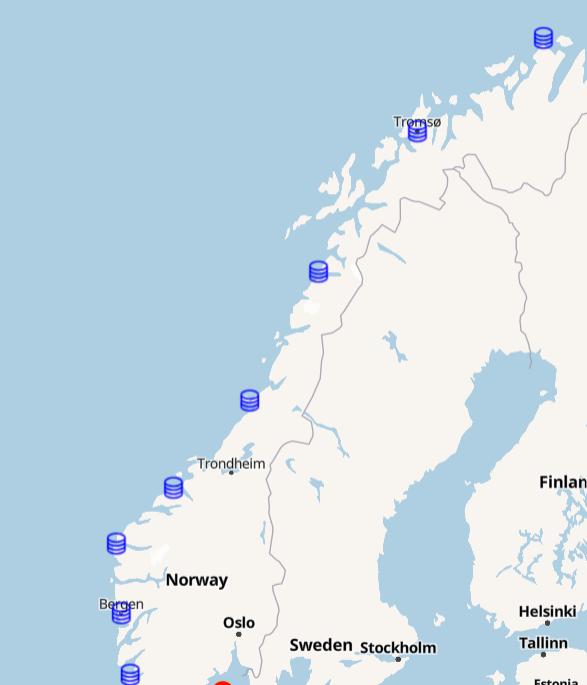
\includegraphics[width=0.4\textwidth,height=0.2\textheight,keepaspectratio]{Figures/Base-station-view.png}
    \caption[Base station layer]{Base station layer showing fixed AIS receiver locations as blue icons, providing persistent geographic reference points on the map}
    \label{fig:base_station_result_image}
\end{figure}
Base stations are linked to anomalies through backend data representing transmissions from individual anomalies. This is then used in other layers to connect base stations to anomalies through signal strength. The base station data itself will never change in position, as they are static points on the map. This provides persistent reference in relation to anomaly and transmitted base station, and helps end users visually observing the distance between anomaly cluster and base station, leading to visual feedback on the spatial relationship between anomalies and base stations.
% SUGGESTION (relocate evaluation — your call): "helps end users visually observing the distance...
% leading to visual feedback on the spatial relationship" is an assessment of usefulness, not an
% observation of the layer. Consider keeping the factual link (base stations are static reference
% points) here and moving the usefulness claim to Discussion.
%TODO Evaluations need to be moved


\subsection{Anomaly Group Visualization}
The anomaly group visualization is shown in Figure~\ref{fig:anomaly_group_result_image}.
\begin{figure}[H]
    \centering
    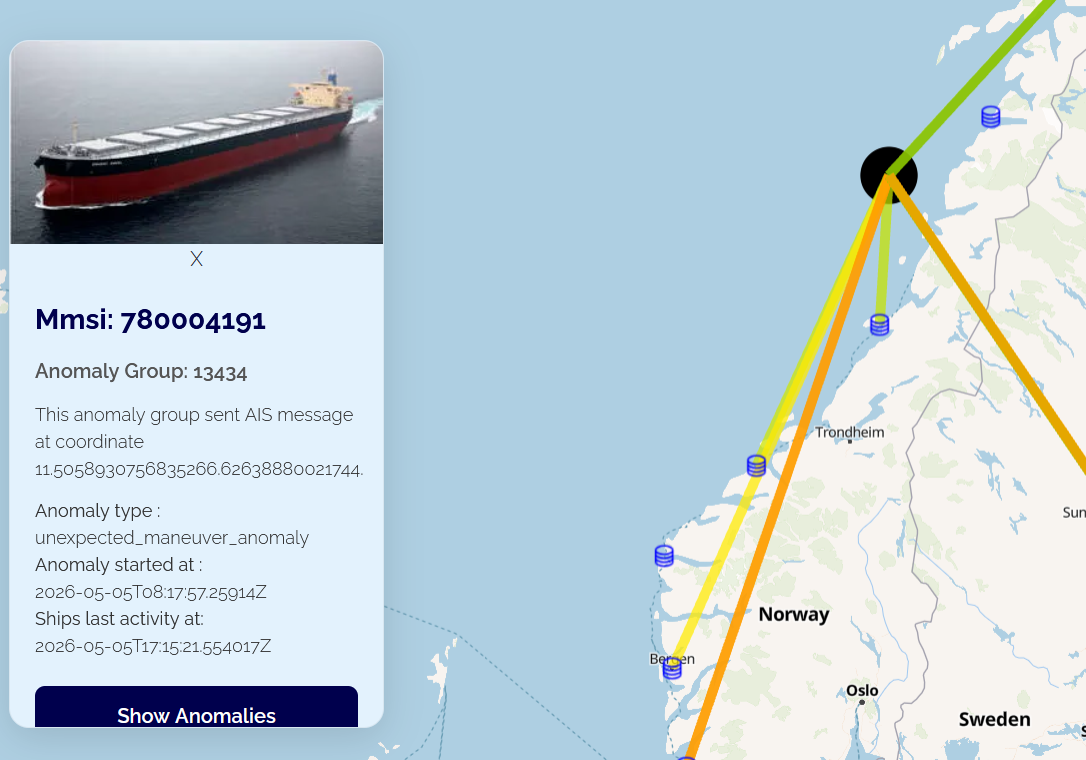
\includegraphics[width=0.8\textwidth,height=0.6\textheight,keepaspectratio]{Figures/anomaly-group-layer-result.png}
    \caption[Anomaly group layer]{Anomaly group layer showing signal strength lines connecting individual anomalies to nearby base stations and satellites}
    \label{fig:anomaly_group_result_image}
\end{figure}

The layer shows an info component for the current group, with coordinates, start date, and anomaly type. Signal strength is visualized through lines, connecting the individual anomalies inside the group to the base stations shown in the picture as blue symbols. The info component allows for users to show anomalies inside the group, through button press on the component, leading to the visualization being changed to the individual anomaly visualization. 


\subsection{Individual Anomaly Visualization}
Individual anomalies are shown as a scatter plot (Section~\ref{sec:scatter_plot}). The visualization shows the points colored based on signal strength, from red to green. This is done through the signal strength value being normalized from 0 to 1, in the database.
% SUGGESTION (Method/Results bleed — your call): "normalized from 0 to 1 in the database" is an
% implementation detail that fits better in Method 3.5. Results can simply state that points are
% coloured from red to green by signal strength.
%TODO Fix this
\begin{figure}[H]
    \centering
    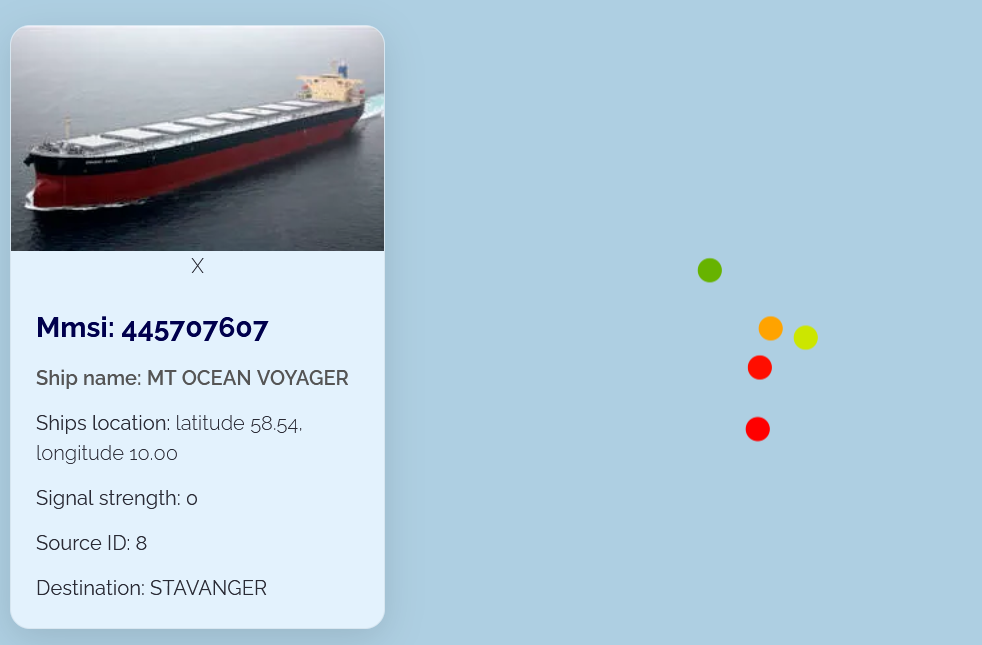
\includegraphics[width=0.54\textwidth,height=0.4\textheight,keepaspectratio]{Figures/individual_anomaly_layer_result.png}
    \caption[Individual anomaly layer]{Individual anomaly layer displaying anomalies as a scatter plot, colored from red to green based on signal strength}
    \label{fig:individual_anomaly_result_image}
\end{figure}
Figure~\ref{fig:individual_anomaly_result_image} shows the completed layer. Anomalies are correctly colored through the signal strength variable, with an info component being shown for an anomaly, through clicking on it. The info component illustrates features of the anomaly, like its direction, name, and MMSI.

% SUGGESTION (4.7 — mirrors Method 3.6;
% YOU still need to: add the screenshots (filter panel, a before/after of the dataset changing, the
% date picker, the satellite layer on click) and expand each description in your own words.
\section{Filter and Interaction}
\label{sec:results_filter_and_interaction}
This section presents the delivered filtering and interaction features, implemented as described in Section~\ref{sec:filter_and_interaction_method}.

\subsection{Filter System}
The filter system allows the rendered dataset to be narrowed by anomaly type, MMSI, and last activity date.
% SUGGESTION (you write/expand): add a screenshot of the filter panel (with a Figure ref) and a
% before/after pair showing the map dataset changing when a filter is applied. State the available
% parameters explicitly.

\subsection{Temporal Filtering}
A date-time range selector allows the visualization to be restricted to a chosen time period.
% SUGGESTION (you write/expand): add a screenshot of the date picker (Figure ref) and describe what
% the user sees when a range is applied.

\subsection{Satellite Visualization}
Satellite connections are displayed as a layer that appears only when a data point is clicked. 
% SUGGESTION (you write/expand): add a screenshot of the satellite layer appearing on click (Figure
% ref) and confirm exactly what triggers it.

\subsection{Interactive Components}
The interface provides interactive controls for selecting filter values.
% SUGGESTION (you write/expand): name the actual controls (e.g. pop-up calendar for dates, dropdown
% for anomaly type, numeric input for MMSI) and optionally add a screenshot.


\section{Testing and Performance}
\label{sec:results_testing}

Testing was done manually, as mentioned in Section~\ref{sec:testing_method}. Console logging and observation based testing was used, to ensure all features work, with performance testing being done through use of the application.
% SUGGESTION (4.8, testing findings — you write it): Method 3.7 has three subsections (Backend API,
% Frontend, Performance methodology) but this produces ~2 sentences of result. Add findings that
% mirror it: (1) a short list of features validated manually (layer switching, filter combinations,
% search, click/info interactions, date range); (2) what the Swagger API testing confirmed (endpoints
% return correct filtered data); (3) bugs found AND fixed during testing (e.g. the cluster-
% recalculation issue mentioned in Method). "Found and fixed" items show the testing did something.

The performance of the system has been observed through rigorous use of the application itself and logging individual parts. Each visualization type was observed at different zoom levels and areas of the map.
% SUGGESTION (de-subjectify — your call): "rigorous" is a subjective qualifier. Consider replacing it
% with what was actually done (which views, which zoom levels, roughly how many runs), and add the
% test hardware (GPU) and dataset sizes so the performance observations below have context.
%TODO Most tests were done with the default zoom with 2-3 refreshes of the website. However for the features that tested clicking of data points they were tested for usually just 2 points to make sure it worked on different points. The hardware utilized was just two labtops utilized by the group for school work. The main data size utilised was 10k points of data, however when testing we usually went up to 100k or 1 million data points. utilizing configs when starting up the backend which creates more template data for more points. The website always rendered data within a second of the request to the backend with most of the time used for sending the request and getting a response. Remaining within a responsive range for the website. By testing was also how we realised we needed a master query to make sure data was queryed all at once and not filtered on the frontend cause of the efficency on the backend.
% Need to get the actual number and some goes in the other subsection

\subsection{Rendering Performance}

The rendering performance is responsive, but will vary based on graphics processing speed of differing computers (Section~\ref{sec:hardware_acceleration}). Rendering happens first with the base map, then with data points, with the other user interface parts appearing with the map. Different visualization methods have different performance, with clustering being faster than heat maps in all cases.
% SUGGESTION (quantify — you write it): add approximate figures if available (dataset sizes tested,
% GPU used, rough layer-switch latency).

\subsection{Effect of Clustering on Performance}
\label{sec:effect_of_clustering_results}

Clustering had a profound effect on the speed of the application, where rendering a scatterplot natively, with over one hundred thousand data points, proved very inefficient. Clustering renders fewer data points, while the same data remains on the actual map. Due to data points being rendered as they are in view, clustering leads to fewer data points being shown while zoomed out, with zooming in showing more data points, while still not being cluttered as a normal scatterplot would be.
% SUGGESTION (quantify — highest-leverage fix, you write it): "profound effect" / "very inefficient"
% are judgments with no number behind them. Replace with a concrete observation you can state even
% from informal testing, e.g. "the plain scatter plot became unresponsive above approximately N
% points, while the clustered view remained interactive." Add the point counts rendered with vs
% without clustering at a given zoom if you have them; move any remaining judgment to Discussion.
%TODO do some actual test on the actual speed of the loading.

\subsection{System Responsiveness}

Responsiveness of the system is observed to be at a satisfactory level, although some operations cost more than others, such as going from a clustered view to an anomaly group view, with signal strength lines being computed, causes some slowdown, but remains responsive after the layer is changed. Other parts of the system like filtering and changing of layers are responsive, and change as soon as input is submitted. The slowest layer is heat maps, as changing zoom or moving around the map, causes it to recalculate the weight of each area. The heat map itself is as responsive as Deck.gl implemented it, leading to no considerable performance gains to be doable, outside of trying to implement a clustered heat map in some way.
% SUGGESTION (relocate evaluation + quantify — your call): "satisfactory level" and "no considerable
% performance gains to be doable" are judgments → move to Discussion. Here, state observed behaviour
% only, and add approximate wait times for the slower operations (e.g. the clustered to anomaly-group
% switch) if you have them.

\section{Customer Feedback}
\label{sec:customer_feedback}

Feedback was collected from two sources through the process described in Section~\ref{sec:user_feedback}: the product owner at Kystverket, and an internal user who works with the AIS analysis system that is closely related to this project.

\subsection{Product Owner Evaluation}

The product owner evaluated the delivered features across four areas: clustering, signal strength visualization, heat map, and the solution as a whole.

\subsubsection{Clustering}

The clustering visualization was assessed positively because it helped provide a proper overview over a large amount of data without the visual clutter. The product owner also noted that clustering is already utilized by other large data systems at Kystverket, however it has not yet been applied to the AIS anomaly monitoring. A suggestion that was given for further development was to be able to display the types and counts of anomalies within each cluster. This would allow operators to assess if further exploring a cluster is worthwhile quickly.

\subsubsection{Signal Strength}

The signal strength visualization was described as a concept they were very interested in. The product owner noted that low signal strength between a vessel and a base station is an error in AIS messages that causes the creation of anomaly messages. Other systems they utilise for signal strength take longer to find the data and do not visualise it properly, increasing the time to analyse anomaly groups and the time complexity for the operator. The delivered solution was assessed as effective both at the macro level, where lines from anomaly groups to base stations are visible while zoomed out, and at the micro level, where individual signal strength values are visible when zoomed in. A suggestion was given to extend the visualization to include additional data like signal strength before and after an anomaly occurs, however this would require additional data from Kystverket.

\subsubsection{Heat Map}

The heat map was assessed to be a useful tool that complements clustering. This was because clustering only shows volume through numbers for large areas and requires zooming in to find areas with large amounts of points, while the heat map is valuable since it allows identification of all the hot spots on a large map at a zoomed-out level without requiring additional work from the user.

\subsubsection{General Solution}

The overall solution was evaluated positively for its features like toggling between visualization types, filtering by anomaly type, and the ability to drill down to the individual anomaly level. The product owner also noted that reimplementing anomaly group and base station views was necessary for the signal strength concept to provide value, even though those views already exist in Kystverket's current system.

\subsection{Internal User Feedback}

An internal user of Kystverket's existing AIS analysis system provided additional suggestions for further development.

\begin{itemize}
  \item Normalizing the heat map against vessel traffic density in
    each area, so that the visualization reflects where anomalies are
    overrepresented rather than where traffic volume is highest.
  \item Extending signal strength visualization to cover all position
    reports from a vessel, not only those linked to anomalies, to
    provide a more complete picture of signal quality over time.
  \item Disabling clustering at low data densities where
    consolidation removes useful detail from the view.
  \item Adding aggregated per-vessel statistics to support long-term
    credibility assessment of individual ships.
  \item Displaying anomaly frequency graphs over time to reveal how
    the situation develops hourly or daily.
\end{itemize}

\section{Project Outcome}

The final project outcome was influenced both by the original project outline and by scope changes introduced throughout development. The implemented system follows the main goals of the original project outline, but has different features implemented as a result of the change of scope.

\subsection{Scope Changes During Development}

During development, and from the start of the project, the project differed in scope from the project outline in subtle ways. All visualization methods that the group worked on were in the project outline, but during the project itself the focus of the application became testing new concepts, such as signal strength visualization, through lines going from anomaly to base station/satellite came later during the project lifecycle. Features such as report generation were not mentioned later in meetings or as a feature request, rather other features were chosen for concept testing. As a result of the scope never being locked down during the project, the customer gave requests on what at a certain point in time would be good to implement to see if value could be gotten in a full implementation in their own software.
% SUGGESTION (relocate evaluation — your call): "As a result of the scope never being locked down..."
% is a judgment that Discussion (Project Execution) already covers. Consider keeping only WHAT changed
% here (features added/removed) and moving the assessment to Discussion.

% Probably create a table for scope here and then for deliverd vs planned

\subsection{Delivered vs Planned Features}

Almost all planned features from the project outline and through meetings were implemented, some being seen as extra features later in development by the customer. A report generating system and satellite orbit visualization feature were not delivered. However satellites themselves were implemented and shown as connected to anomalies through a signal strength line in the anomaly group layer, showing its position at the time of data transmission. The overall delivered features implement the majority of the project outline's features, while also implementing the requested features from the customer.
% SUGGESTION (table + måloppnåelse honesty — you write it): replace this paragraph with a table —
% Feature | Status (Implemented / Partial / Not implemented) | Notes — listing EVERY objective from
% the Introduction, including shortfalls. The audit flags three to list honestly: Temporal Analysis
% "forward and backward in time" (Intro) -> delivered only a date-range filter = PARTIAL; hexagonal
% binning (project brief) -> NOT implemented; satellite orbit plotting -> NOT implemented. A sensor
% cross-checking the Introduction against Results will catch omissions, so list them.


%TODO Move this to the other one.
% SUGGESTION (relocate whole section to Discussion — your call; Discussion lives in 07Discussion.tex,
% out of my current scope): this entire section is comparative EVALUATION, not a result. Consider
% moving it wholesale into Discussion. If it stays here, it caps how factual the Results chapter reads.
\section{Comparison to Customer's Tools}

As the resulting application is testing concepts for the customer, a direct comparison yields little value, as the customer themselves mentioned that the currently in use tools are superior in their core functionality. However as the currently implemented application is testing new visualization methods and features, this then brings value to the customer to test if their already in use software, or software they are to make themselves, should have these features. As a result the software created for the project is better in the specifics of testing new concepts.

%=====================================================================
\cleardoublepage


\chapter{Discussion}

%=====================================================================
\textit{This chapter evaluates the finished project and reflects on the technical, methodological, and contextual factors that shaped the outcome.}

\section{Overview of End Product}

The finished product meets the main requirement the customer requested, with few features from the original project description being omitted. The quality of the finished project as a concept test for new visualization methods was noted in the customer feedback presented in Section~\ref{sec:customer_feedback}.

The overall solution was assessed as satisfactory by the customer, as it allowed them to test concepts of new visualization modes like signal strength, clustering, and heat map layers. Collaboration with the customer was effective troughout the project, with frequent communication supporting the addition of new features and the resolution of technical questions as they arose.

The project demonstrates that visualization of large datasets through methods not currently in use by the customer can provide concrete value. This is reflected in the customer's stated intention to incorporate several of these features into their existing software.

\section{Discussion of Technical Solution}

The technical solution, described in Section~\ref{sec:system_architecture}, is documented and functions as intended, with emphasis on simplification through the use of helper classes and repeated refactoring throughout the project.


\subsection{System Architecture}

The system architecture, with Deck.gl overlaid on MapLibre as the base map and a Docker-based backend providing data, worked well throughout development. The modular approach led to MapLibre being separated from the Deck.gl implementation (Section~\ref{sec:deckgl}), with the map itself responsible only for  map-related functionality such as zooming and movement. This separation simplified the overall complexity and produced cleaner code with a clear separation of concerns. Achieving this required a period of refactoring tightly coupled code, particularly where the map itself contained functionality unrelated to its task. 

The architecture choice was partially guided by the customer, whose request to use React and other technologies already in use within their infrastructure shaped the group's decisions, alongside with the customer providing the backend. Maplibre was suggested in the project document and was ultimately selected as the map provider, supported by its open-source nature and use of vector tiles (Section~\ref{sec:vector tiles}).

\subsection{Frontend}

The frontend implementation successfully followed the wireframes established at the beginning of the project (Section~\ref{sec:design_process}). The design is minimalist by comparison to other applications, prioritizing the map and visualization components over additional interface elements. 

The choice of map provider had both advantages and disadvantages. Maplibre is a fork of the now closed-source Mapbox, which meant that documentation was less comprehensive than required, and that more detailed information for equivalent code often had to be retrived from the Mapbox website. As a result working with MapLibre required more time spent understanding the library than was originally anticipated, delaying implementation beyond what had been planned.

Deck.gl (Section~\ref{sec:deckgl}) proved to be an effective choice for visualization, providing all functionality needed to implement the customer's requested features. Layering through Deck.gl allowed straightforward integration with MapLibre by utilizing a MapBox-style overlay. Since MapLibre is a fork of MapBox, no additional integration code was required beyond what would have been needed for MapBox itself. 

% Needs to be fully rewritten/ add more context since we have experience, just not the knowledge needed for developing a map based application and the logic that should be used as well as standards.
The use of React with TypeScript enforced stronger type safety than plain React, but introduced an initial learning curve. The group's lack of experience with the coding standards needed for react and typescript, led to development time being spent on learning the basics as well as more advanced tools such as Context, which was ultimately used to simplify the code.  

The single-page design, which covered all required functionality through interactive components, suited the project well. One advantage over a multi-page architecture, was that the map and visualization remained visible at all times, including during manual testing of other components. The overall simplicity of the interface also aligned with the projects focus on concept testing, particularly as the customer themselves had requested that less time would be spent on design and more on functionality.
 

Overall, the frontend implementation fulfilled the project's main goals while highlighting how the use of third party tools can present challenges, and how tool selection is an important step in any software development project. 


\subsection{Visualization Methods and User Interaction}

The chosen visualization methods were effective for different aspects of anomaly visualization, each with their own strenghts and weaknesses related to readability, performance and interaction. 

% TODO: Add the date for change in efficeny for clustering and singular scatter plot.
Clustering, implemented as described in Section~\ref{sec:clustering_method} and shown in Section~\ref{sec:effect_of_clustering_results}, produced a measurable performance improvement compared to a normal scatter plot of all points in the dataset, while also improving readability. 

The zoom function with layer recalculation was observed to remain responsive during manual testing, although responsiveness remained dependent on the hardware running the application. The layer was implemented with a focus on simple visualization, including a numeric label indicating count of anomaly groups within each cluster, presented in a clear and readable manner. The layer is also interactive, with pressing 
% Might need to be rewritten cause it is easily misunderstood.
a single individual anomaly group cluster leading to the anomaly group layer, this is performant through api call to the backend, instead of acquiring the information through frontend filtering. The main drawback with clustering is the lack of specific details of each anomaly group, requiring multiple layer changes to go into an anomaly group and then into the individual anomalies, it gives a generally simpler overview of where anomalies are grouped, and how numerous they are, but no specific details on the anomalies inside. Although this is worth the tradeoff versus having a normal scatterplot with a chaotic amount of points shown at once. 

The Heat map visualization, implemented as described in Section~\ref{sec:Heat_Map_method}, provides value by representing the entire dataset, rather than the aggregated form used by clustering. This produces a overview of all data points based on proximity, in contrast to clustering visualization, it utilizes color intensity to represent hot spots more precisely. Color based encoding is more visually intuitive for identifying hot spots compared to visually identifying density based on size and numeric labels. This benefit also justifies higher rendering costs utilized by heat map's. This means the visualisation method is slower than other methods while it offers a more comprehensive overview of the dataset. % TODO: add data here or in results for rendering times like for clustering and induvidual scatter plot.

The anomaly group layer, described in Section~\ref{sec:anomalies and anomaly groups}, provides detailed information about each individual group. The signal strength visualization is central to this layer, and the implementation received positive feedback from the customer (Section~\ref{sec:customer_feedback}). The combination of location, anomaly type, and connections to base stations and satellites in the information component,provides a clear overview of how an anomaly group relates to the receivers of AIS messages. 

The individual anomaly layer, implemented as a scatter plot (Section~\ref{sec:scatter_plot}), was added at the customer's request, with an info component being used to display the data properties of each anomaly. The layer provides further insight into the individual anomalies within a group, including their heading and signal strength. The layer adds clear value to the project and presents no significant drawbacks. 

The remaining visualizations, including the base station layer (Section~\ref{sec:base_station}) and the satellite layer, are required for layers such as the anomaly group with signal strength to provide any useful information. They are therefore crucial too the project and presents no notable drawbacks in their implementation. 

User interaction is a core part of the application, and user's should be able to navigate and retrieve information without noticeable slowdown or errors. Based on manual testing during development, user interaction was observed to remain responsive, even though performance remains heavily dependant on hardware used, with the available GPU acting as the main limiting factor for rendering performance (Section~\ref{sec:hardware_acceleration}).% TODO: Add measured data for interaction latency

Actual user interaction is based heavily around the zoom and camera location of the application. This interaction with the map has drawbacks such as performance loss, but allows for information on anomalies, filtering and searching. This user interactivity comes with the downside of the performance loss, with system responsiveness being affected. As a core feature of the application, the trade of with responsiveness and performance are offset, with non static datasets being much easier to analyse. 


\subsection{Backend and data handling}

The backend being provided by the customer, has comprehensive documentation of endpoints through swagger, with all the endpoints needed for the project implemented. Docker proved to simplify the process of running the backend, with few sentences of code being required to start and fill the database with test data. Observing the backend performance showed no critical performance or data errors, but the delivered backend itself comse with limitations on being constrained to the predefined API structure, with extensions being more complicated for the group to implement themselves, due to lack of experience with the programming language GO. Although the observed performance was satisfactory, testing of the performance was not controlled by the group itself, with core negatives of the backend implementation being wait time for customer to implement required features, a less often occurrence. As a result the backend was well implemented, but not controlled solely by the group, this being a tradeoff.

Data handling through GeoJSON, proved a good choice for both the backend and frontend, with the libraries used already supporting the data. The data itself being parsed through a deck.gl layer. The layer being responsible for parsing data from each GeoJSON feature. Proved to be an effective design, that allows for simple access to data, through accessing properties and geometry of said features. A tradeoff of using GeoJSON is that the frontend must have prior knowledge of the data structure in order to correctly access said properties and geometry. This introduces dependency on a clear schema. Another issue with data, has been asynchronous errors, with wrong data being delivered, or data being accessed before delivery. 
  
%=====================================================================

\section{Performance and Scalability Discussion}

The performance of the system is highly dependent on hardware specifications, with particular effect coming from GPU capability. Webgl has highest effect on greater GPU's, leading to performance being bottlenecked on weaker systems. 


\subsection{Rendering Performance}

Base rendering performance of maplibre, is observed to not have issues, with performance being taxed on the visualization methods and dataset size, rather than the map. Datasets were tested from thousands, to over one hundred thousand, with both having little issues on group computers. The architectural design of the project is not bottlenecked based on the backend, but with frontend using supercluster to recalculate clusters based on zoom, and similar calculations being done on heat map, leads to zoom and move operations being most taxing on the system. This can be tweaked to recalculate fewer times on zoom level, but will lead to a less responsive system. The core bottleneck of any performance is then the frontend itself, with the backend being called in milliseconds. 


%=====================================================================

\section{Project Execution}

This section evaluates the project management process described in Section \ref{sec:dev_methodology}, focusing on how the chosen methodology, team structure, and communication practices influenced the development outcome.

Although the adopted methods ensured a structured development process, several of them introduced weekly overhead that proved disproportionate for a two-person team operating under a fixed deadline. The following subsections evaluate each aspect individually.

\subsection{Scrum Framework and Sprint Structure}

The Scrum framework provided a consistent structure for planning and delivery. The system was designed for large groups, so it had issues in relation to workload and redundancy for groups of two. Therefore, the daily stand-up system was altered and implemented to occur multiple times a day instead to make sure the group had proper accountability and focus in relation to scope. It also helped keep motivation high and allowed the group to quickly make changes to tasks depending on problems found with them. Instead of the standard two-week sprint, the group used weekly sprints as well, to supplement issues which were fixed by multiple daily stand-ups. Since it was a group of two, the focus of the project and scope were defined and worked toward each week while also making sure the backlog was handled.

However, several Scrum artifacts introduced documentation overhead that provided limited value at this team size. This became a bigger issue because of the decision to have weekly sprints, which increased the overhead that needed to be handled compared to the standard system. The problem was amplified because sprints documented and reviewed the backlog every week, even though group members had continuous visibility into task status through GitHub Projects.
 % Maybe ref or  section

In relation to sprint documentation, the sprint artefacts provided traceable project documentation, which served as a reference when writing the report while ensuring important information was not lost in miscommunication.

\subsection{Team Composition and Workload Distribution}

In a group of two where both members had mostly the same knowledge and expertise, workload was distributed based on member preference and the nature of each task, which made documentation responsibilities formally split where one member handled the sprint documentation while the other handled meeting documentation while development tasks were shared. In practice however, more demanding tasks were rotated between members to maintain motivation. This type of informal balancing worked well for a group of 2 but would not scale to a larger team, where responsibilities would be split more evenly with explicit role definitions. 

\subsection{Communication and Meeting Structure}

Slack provided an efficient channel for direct communication with the customer, enabling rapid resolution of short technical questions. The customer's domain expertise allowed complex questions to be resolved within short discussions rather than through a long discussion. While communication with the supervisor was handled primarily through email, with in person consultations used for urgent issues, because most work was conducted on campus.

For meetings, biweekly meetings were held with both the supervisor and the customer at Kystverket. Before these meetings, discussions were held to discuss which questions should be asked. However, most of these discussions happened through a small meeting before the actual meeting or through daily stand-ups within the group.

Most meetings with the customer were focused on whether the customer liked what had been developed, followed by technical questions to figure out the difficulty of harder problems and what they wanted the group to focus on. With the supervisor, however, problems relating to documentation and any issues with what had been done were mostly discussed. There were sometimes occasions where meeting times were delayed because the customer was busy or had taken a break from work.

\subsection{Task Management and Version Control}

The task management infrastructure described in Section \ref{sec:task_management} worked effectively for the project, although the multi-repository setup introduced some context-switching overhead. The four workflow stages would have been more useful in a larger group, however since work was handled in person they served mainly to track which tasks had not been done or which member was currently working on each task. The three-repository structure occasionally caused issues to be filed in the wrong board, where they were overlooked until rediscovered and relocated. The burndown chart was generated automatically and used to track project progress and identify whether the project was accumulating unaddressed issues. The three-board structure worked better than a single combined board, because GitHub Projects allowed all three to be viewed together at the overview level while keeping each repository's issues separated at the detail level.

For version control, Git was utilized because it allows code to be reverted easily if new code breaks the system or creates unexpected issues. Branching was useful overall, even though it occasionally caused merge conflicts and required refactoring after code was combined. This was still preferable to working in a single shared branch, where both members would have caused conflicts continuously during development.

\subsection{Scope Management}

Scope management was handled reactively through customer meetings rather than through a formal change process, which had both benefits and drawbacks. The weekly sprint cycle allowed scope changes to be incorporated quickly, which was valuable given the short development period and limited team capacity. This approach kept development aligned with the customer's interests and prevented time from being spent on challenging features that were not needed. However, the absence of a formal scope freeze meant that new requests led to planned features being cut to accommodate them. The reactive approach worked well within the constrained timeline, although a longer project would have permitted more features to be properly developed and polished. For a project of similar length, a formal scope freeze date would improve predictability. Weighted prioritization could also help larger teams manage competing requests, but the small team size and direct communication with the customer made this less necessary in this project.

% Should be in technical solution and discussion of that since 
\begin{comment}
\subsection{Code Quality and Maintainability}

The code quality was designed to follow software principles, but due to lack of experience with react itself, some uncertainties about use of specific methods arose. The use of prior programming experience to create files that handle specific tasks, are however used to simplify the program, with refactoring being done multiple times to follow these guidelines

\subsection{problems during development}

Multiple problems arose during the development of the project. A core problem being the changing of the scope throughout the project, which lead to features being cut in focus on new features being added.This was handled through communication with the customer, where functionality to focus on was honed in on. 
\end{comment}

%=====================================================================

\section{Limitations}

Although the project fulfilled the main end requirements through scope changes that the the customer requested, it still has limitations and is a concept testing software. 

\subsection{Technical Limitations}

Technical limitations include not having implemented real AIS data from the customer in the project. This would be unlikely to have happened with any amount of work on the project as such information is classified, resulting in it being something the customer can take forward themselves. Other limitations are satellite orbit not being plotted, as was a request that was given, but not able to implement in time. This would have allowed for users to see the orbit from the satellite, from its current position, to its positions in the future. Although satellite orbit was not implemented, satellites themselves were, and show up in the signal strength visualization. Another feature from the project outline not implemented, that was quietly removed from scope, is automatic report generation, but this was removed as a request in the project, where focus went into concept testing. 




%=====================================================================
\cleardoublepage


\chapter{Conclusions}

\textit{This chapter summarizes the project, revisits the objectives, and reflects on the overall outcome of the developed system}


The goal of the project was to evaluate whether alternative visualization methods and features could provide new value to the Norwegian Coastal Administration, in analyzing \acrshort{ais} anomaly data. The focus was on developing a prototype application that enables analysis of large-scale anomaly data sets through interactive filtering and multiple new visualization approaches. 


The final system demonstrates a locally hosted prototype allowing for analysis of \acrshort{ais} anomaly data. It allows users to view anomaly patterns through clustering, heatmap visualizations and detailed inspection of anomaly groups and individual anomalies. In addition, filtering based on \acrshort{mmsi}, anomaly type and date range were added to enable a targeted analysis of anomalies and their connection to base station and satellites. Together, these features support a high level view of where anomalies aggregate, and their signal connection to base stations on the coast alongside satellite representation. 

The project demonstrates that it is possible for third party tools and modern web technologies to prototype new features and methods in data analysis. This approach enables early evaluation of visualization concepts without requiring full scale development on these systems, allowing verification of the concepts value and reducing development risk, and unnecessary time usage. 

The project objectives were in large part achieved, fully implementing the core visualization and interaction features requested, including clustering, heatmaps, filtering and information components, alongside signal strength and individual anomaly layers. However, some planned features, such as hexagonal binning, more complex visualization of satellite orbits, and report generation, were not implemented due to time constraints and scope cuts that kept focus on the delivered system.
% SUGGESTION (criterion 5 rewards an explicit goal-by-goal verdict): consider walking the four
% Introduction objectives (Advanced Map Visualization, Data Aggregation/Clustering, Temporal Analysis,
% Efficient Querying) and stating met / partially met / not met for each. Temporal Analysis was only
% partially met (date-range filter, not forward/backward animation) -- saying so explicitly scores
% better than a general "in large part achieved".

Further improvement could be implemented, such as integration with the customers real-time \acrshort{ais} data stream, to enable monitoring of live data. More advanced temporal analysis or implementation of cut features such as hexagonal binning, can add new value to the system. The system can also be further worked on to visualize more than \acrshort{ais} data, and can be used to test concepts related to other fields and visualization methods. 

Overall, the implemented system meets the main objective of creating a simple, readable visualization program for \acrshort{ais} anomaly data, while remaining open for further work. 




\cleardoublepage

\chapter{Societal Impact}
\textit{This  chapter discusses the societal and economic consequences, or lack thereof the project contains, while discussing sustainability and environmental sides.}

\section{Societal and Ethical Impact}


In communication with the customer on societal and ethical impact, key insights were given. Better visualization of AIS anomalies, is a tool that would transform how current work is done, rather than remove employment opportunities, leading to specialized workers, with access to more effective tools. As such the workplace impact of a fully developed software would not have a negative impacts on workers, neither would the use of better tools lead to loss of employment. As the system would be used to analyze data from large vessels, small vessels would not be affected by this. As a result no surveilance of individual persons would be committed if the tool was connected to real data. A fact of this is that boats are required to use AIS transponders by law, leading to the system not being a new form of surveillance on sea vessels. Another point raised in talks with customer is around the scenario if this could be used to stop illegal smuggling or immigration, but the vessel type being large, means the likelihood of this is low, as large vessels are less suited for illegal tasks like smuggling. 


\section{Economic}


The prototype itself, proves that feature testing can be used to see value, or lack thereof in new features and systems. This can reduce financial risk through not implementing wasted features, leading to less negative consequences economically. Also the use of open source tools cut down on licensing and other costs, leading to the prototype being a financially viable way of testing new systems and features. 

\section{Sustainability}

The sustainability impact of a software development project is generally low. The project itself can reduce wasted effort implementing features not needed. THE system itself can be extended and is maintainable for other developers to work on, leading to a scalable and maintainable system. 


\section{Environment}

The software not requiring physical components aside from computers, leads to very low emissions. And only electricity being required to run the software. Improved AIS detection could lead to action being taken sooner on faulty boats, leading to reduced environmental impact. The software itself can then not have a large amount of environmental impact. 
\cleardoublepage




\addcontentsline{toc}{chapter}{\protect\numberline{}References}
\printbibliography[title={References}] %you may change the title in the toc here if you want
\cleardoublepage


\chapter*{\LARGE \textbf{Appendices}}
\fancyhf{} %clear the header, it should be empty for the appendices
\renewcommand{\headrulewidth}{0pt} %no rule
\fancyfoot[C]{\thepage} %page numbers centered in the footer
\addcontentsline{toc}{chapter}{\protect\numberline{}Appendices:}
\appendix


\chapter*{A - Github repository}
\addcontentsline{toc}{chapter}{\protect\numberline{}A - Github repository} 

All code and latex-files used in this document are included in the Github repository linked below. Further explanations are given in the readme-file. 




%=====================================================================
% Make every defined abbreviation and term appear in the Abbreviations and Terms
% lists, even entries not referenced with \acrshort/\gls in the body (e.g. CPU,
% VTS, JSON, and all glossary terms). Without this the Terms list would be empty.
% Placed at the very end of the document so entries used earlier keep their real
% page numbers; only genuinely unused entries are added without a location.
% (This can be moved to main.tex just before \end{document} if you prefer.)
\glsaddallunused


%%%%%%%%%%%%%%%%%%%%%%%%%%%%%%%%%%%%%%%%%%%%%%%%%%%%%%%%





%%%%%%%%%%%%%%%%%%%%%%%%%%%%%%%%%%%%%%%%%%%%%%%%%%%%%%%%


% Register any abbreviations/terms that are defined but not referenced in the body, so they still
% appear in the Abbreviations and Terms lists. Must run before \end{document}; placed last so entries
% used earlier keep their real page numbers and only genuinely unused entries are added without a location.
\glsaddallunused


\end{document}
